\section{Le concept de l’entropie}

	\subsection{À quoi sert l’entropie ?}
	
		Au tout début du \coursun, nous avions vu que nous pouvions conceptualiser l’\vocab{énergie} comme étant «~une grandeur qui ne varie jamais lorsque les choses évoluent~». Ainsi, nous utilisons les quantifications de l’énergie pour déterminer les limites du possible : par exemple, nous savons qu’avec~\SI{500}{\joule}, un corps immobile de masse~\SI{10}{\kilogram} ne peut pas accélérer au-delà de~\SI{10}{\metre\per\second}.
	
		Pourtant, notre intuition et notre expérience quotidienne nous apprennent que beaucoup de transformations ne peuvent avoir lieu que dans un seul sens (\cref{fig_water_jump}). Par exemple, il y a autant d’énergie dans un verre d’eau au rebord d’une table que dans ce même verre brisé avec cette même eau renversée sur le sol. Pourtant nous savons, ou plus exactement, nous avons la conviction profonde, qu’il est \emph{possible} que le verre tombe et se casse, mais \emph{impossible} que les éclats et l’eau sur le sol se rassemblent spontanément en un verre plein sur la table.\\
		Ainsi, la quantification de l’énergie n’est pas entièrement suffisante pour déterminer \emph{ce qui est possible}. Nous souhaiterions pouvoir en plus prédire de façon absolue et quantitative le sens dans lequel l’énergie peut ou ne peut pas être transformée.
		\begin{figure}
			\begin{center}
				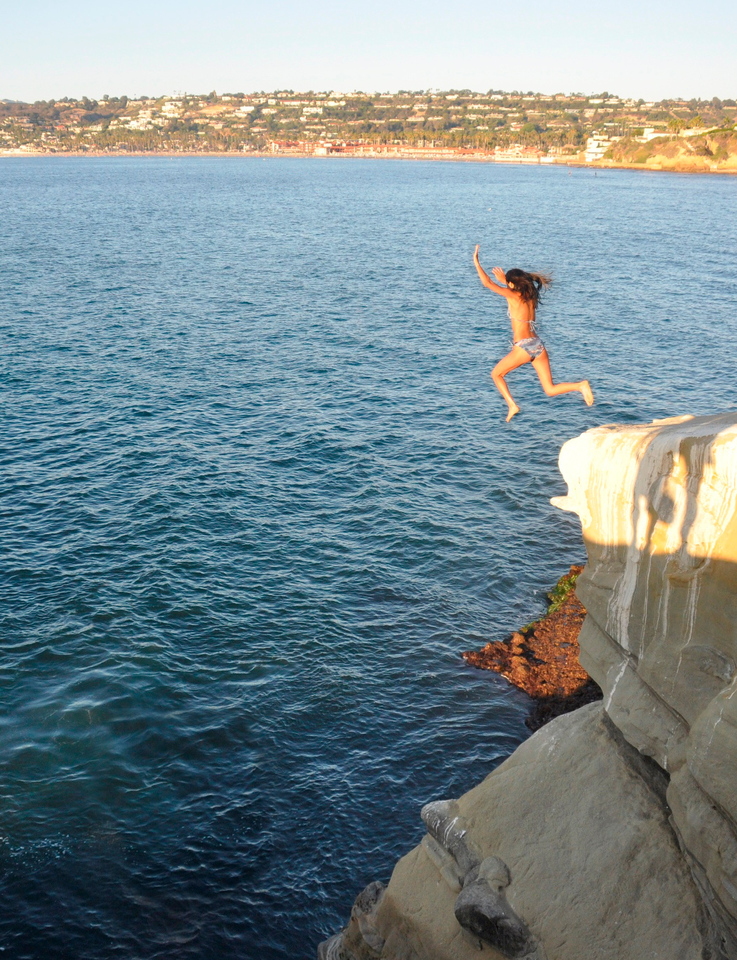
\includegraphics[width=0.31\textwidth]{images/water_jump_1.jpg}
				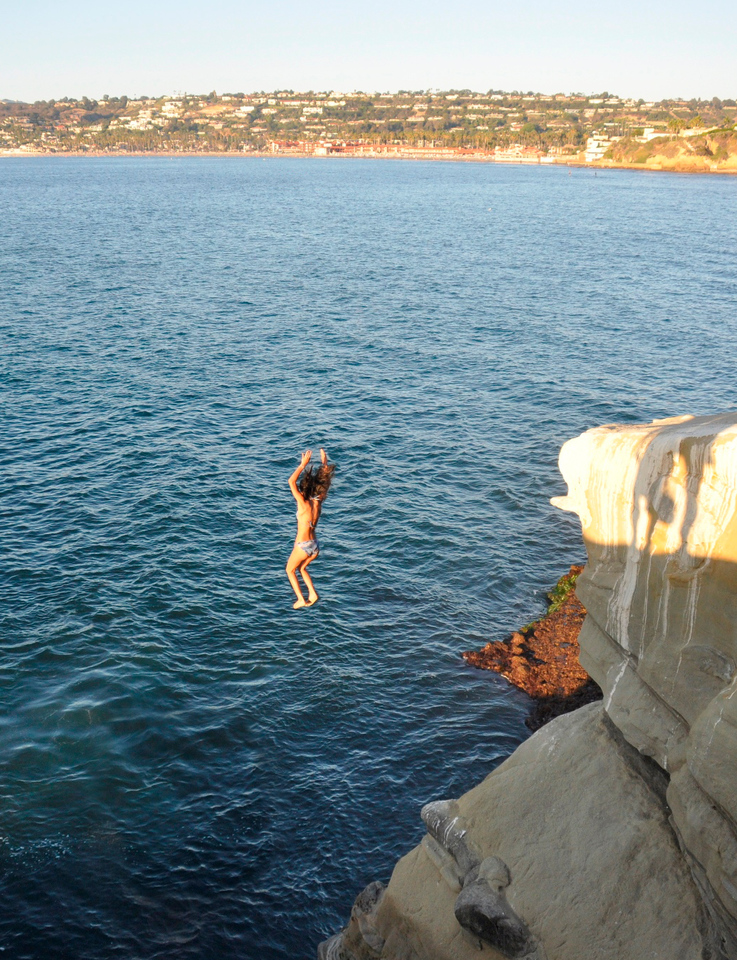
\includegraphics[width=0.31\textwidth]{images/water_jump_2.jpg}
				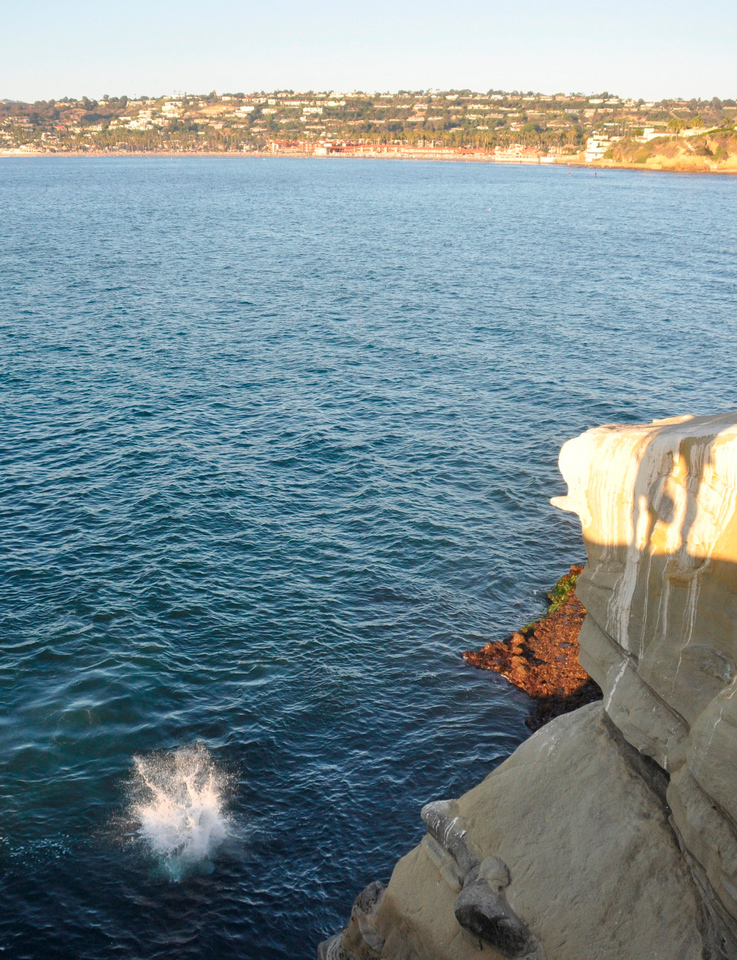
\includegraphics[width=0.31\textwidth]{images/water_jump_3.jpg}
			\end{center}
			\supercaption{Nous avons l’intuition et une intime conviction que ces trois photos ont été prises dans un ordre bien particulier. Une mesure de l’\vocab{entropie} dans ces trois situations, dans lesquelles l’\emph{énergie} est la même, nous permet de déterminer cet ordre en associant à notre intuition une grandeur calculable.}{images dérivées de \wcfile{La Jolla Cove cliff diving - 02.jpg}{photos} \ccbysa par \wcun{Jarekt}{Jarosław W. Tuszyński}}
			\label{fig_water_jump}
		\end{figure}
	
		L’\vocab{entropie} a été pensée pour répondre à ce questionnement. À la fin de ce chapitre, nous disposerons d’un outil permettant de \emph{calculer} le sens d’une évolution, c’est-à-dire de prédire mathématiquement laquelle de deux situations séparées dans le temps doit avoir eu lieu avant l’autre.

	\subsection{Comment déterminer le sens d’une transformation ?}
	
		Dans le vocabulaire de la thermodynamique, le concept d’une «~évolution à sens unique~» est bien sûr nommé \vocab{irréversibilité}. Nous avions déjà abordé l'irréversibilité en section \S\ref{ch_évolutions_irr_sf}, où nous avions déterminé qu’elle avait deux causes principales :
			\begin{itemize}
				\item La transformation d’un travail en chaleur, par frottement et turbulence ;
				\item La transmission d’une quantité de chaleur entre deux corps de température différente.
			\end{itemize}
		
		Les transformations irréversibles dans les fluides conduisent invariablement à des états où la température, la pression ou le volume sont plus grands qu’ils ne l’auraient été avec une transformation réversible. 
		
		\thermoquotebegin{O}
			Pour cela nous imaginons qu’après la transformation que nous souhaitons étudier de cette façon, la masse est ramenée à son état initial par une opération réversible. De cette façon, nous obtenons un petit processus cyclique, à laquelle l’équation (II) s’applique aussi bien qu’à l’ensemble. Si [le long de ce processus] l’on connaît également les quantités de chaleur qu’a reçu la masse pendant ce dernier ainsi que les températures auxquelles elles correspondent, alors l’intégrale négative $-\int \frac{\diff Q}{T}$ nous donne la transformation non-compensée impliquée pendant celui-ci.
		\thermoquoteend{Rudolf Clausius, 1856~\cite{clausius1856, clausius1867en,clausius1868fr3}}{}
		Pour quantifier l’irréversibilité d’une évolution, nous allons quantifier \emph{la chaleur qu’il faudrait retirer au corps pour le ramener dans son état initial de manière réversible}. En lui soustrayant la chaleur qui a été effectivement transmise, nous obtenons en quelque sorte la chaleur qui a été inutilement créée pendant l’évolution.\\
		Or, plus la température à laquelle cette chaleur créée est basse, moins elle peut être transformée en travail (\S\ref{ch_efficacité_moteur_carnot}). Nous allons ainsi «~pénaliser~» le coût en chaleur en le divisant par la température.
		
		De cette manière, nous allons obtenir une grandeur en \si{joules} par \si{kelvin} --\ l’entropie créée pendant l’évolution\ -- qui va être nulle pendant les évolutions réversibles, et qui va toujours être positive pendant les évolutions irréversibles. C’est cette création qui sera le signe manifeste que la transformation n’est possible que dans un sens. %"manifeste" pour "unmistakable", "que l’on ne peut pas ne pas reconnaître". hmmm...

\section{Définition}

	\subsection{L’entropie est une propriété}
	\label{ch_entropie_propriete}
	
		Commençons par admettre le fait que l’entropie est une \vocab{propriété} physique\footnote{On dit aussi \vocab{variable physique} ou \vocab{variable thermodynamique}.}, c’est-à-dire quelque chose qui caractérise l’état d’un système. Dit autrement : si l’on considère une portion de l’univers à un moment donné (un système), nous trouvons que ce système a une masse, un volume, une température, etc. : ce sont ses propriétés, des descriptions absolues de son état. L’entropie est une de ces propriétés.
		
		Par contraste, nous pourrions dire que la chaleur, le travail, le courant électrique etc. ne sont pas des propriétés : ce ne sont pas des quantités qui décrivent un objet, mais plutôt un transfert entre deux objets.

		Nous penserons donc toujours à l’entropie comme étant l’entropie «~\emph{de quelque chose}~» (peut-être comme nous dirions la couleur, la température «~de quelque chose~»). Nous dirons par exemple «~ce corps a de l’entropie~» ou «~l’entropie de ce corps augmente/diminue~», et non pas «~nous prenons/donnons de l’entropie à ce~corps~».
	
	\subsection{Définition}
	\label{ch_entropie_definition}
	
		On nomme \vocab{entropie} une propriété physique notée $S$.
		
		\begin{itemize}
			\item Lorsqu’un système suit une évolution réversible, son entropie varie de façon telle que :
				\begin{equation}
					\diff S \equiv  \left( \frac{\diff Q}{T} \right)_\text{rév.}
					\label{def_entropie}
				\end{equation}
				{\small%handmade, pour éviter trop de retours à la ligne
				\begin{equationterms}
					\item où l’indice \textit{rév.} spécifie que le calcul se fait le long d’un chemin réversible ;
					\item 	\tab $\diff S$ 	\tab est la variation infinitésimale d’entropie (\si{\joule\per\kelvin}) ;
					\item 	\tab $\diff Q$ 	\tab est la quantité infinitésimale de chaleur fournie de façon réversible (\si{\joule}) ;
					\item et \tab $T$				\tab\tab est la température à laquelle a lieu le transfert de chaleur (\si{\kelvin}).
				\end{equationterms}
				}

				Lorsqu’il passe d’un état A à un état B de façon réversible, l’entropie d’un système varie donc d’une quantité $\Delta S$ :	
				\begin{equation}
					\Delta S = \int_\A^\B \left( \frac{\diff Q}{T} \right)_\text{rév.}
					\label{eq_variation_franche_entropie}
				\end{equation}
				\begin{equationterms}
					\item où l’indice \textit{rév.} spécifie que l’intégration se fait le long d’un chemin réversible.
				\end{equationterms}

			\item Lorsqu’un système suit une évolution irréversible entre A et B (comme pour la majorité des évolutions réelles), alors \emph{il faut trouver un chemin réversible entre ces deux états} et y effectuer l’intégration~\ref{eq_variation_franche_entropie} pour calculer $\Delta S$. 

				Il existe toujours une façon réversible (en fait, il existe même une infinité de façons) de faire évoluer un système entre deux états quelconques. Pour cela, il faut que le travail qui lui est transféré le soit de façon infiniment lente, et que la chaleur qui lui est transférée le soit avec une différence de température infinitésimale.
				
				Attention : si l’on intègre la quantité $\frac{\diff Q}{T}$ le long d’une évolution où la température ou la pression ne sont pas homogènes (par exemple lors d’une détente rapide, d’un réchauffement hétérogène ou d’un gradient interne de température, cf. \S\ref{ch_évolutions_irr_sf}), alors on obtiendra un résultat plus faible que $\Delta S$, la variation d’entropie réelle. 
				
			\end{itemize}


		L’unité de l’entropie, $S$, est le \si{\joule\per\kelvin} (\si{joule} par \si{kelvin}) ; et de façon correspondante, on définit l’\vocab{entropie spécifique} $s$ :
		\begin{equation}
			s \equiv  \frac{S}{m}
		\end{equation}
		\begin{equationterms}
			\item où \tab $m$ \tab est la masse considérée (\si{\kilogram}),
			\item et \tab $s$ \tab est son entropie spécifique (\si{\joule\per\kelvin\per\kilogram}).
		\end{equationterms}

		En pratique, le terme «~entropie~» est souvent utilisé même s’il s’agit d’entropie spécifique ; le symbole et le contexte permettent de déterminer à quelle variable il est fait référence.

		\begin{anexample}
		\label{exemple_delta_entropie_basics}
			On prélève \SI{2000}{\joule} sous forme de chaleur, de façon réversible, à une masse d’air en maintenant sa température constante à \SI{30}{\degreeCelsius}. De combien varie son entropie ?
				\begin{answer}
					Comme l’évolution est réversible, nous appliquons immédiatement l’\cref{eq_variation_franche_entropie} : $\Delta S 
						= S_B - S_A
						= \int_\A^\B \left( \frac{\diff Q}{T} \right)_\text{rév.} 
						= \left[\frac{1}{T_\text{cste}} \int_\A^\B \diff Q \right]_\text{rév.}
						= \left[\frac{1}{T_\text{cste}} Q_\fromatob \right]_\text{rév.}
						= \frac{1}{\num{30} + \num{273,15}} (\num{-2000})
						= \SI{-6,6}{\joule\per\kelvin}$.
					\begin{remark}Nous avons déjà exploré les évolutions réversibles à température constante (isothermes) aux sections \S\ref{ch_gp_isothermes} et \S\ref{ch_lv_isothermes}. Ici le gaz perd \SI{2}{\kilo\joule} de chaleur et reçoit \SI{2}{\kilo\joule} de travail.\end{remark}
					\begin{remark}Nous ne connaissons pas la valeur de l’entropie, mais nous savons qu’elle diminue de 7 \si{joule} par \si{kelvin}.\end{remark}
					%Attention dans le rendu PDF le mot "joule" n'est *pas* au pluriel. Je suppose que c'est une convention de notation en physique, je trouve que ça choque tout de même à la lecture (d'autant que dans d'autres occurrences dans l'ouvrage, joule est au pluriel)
					\begin{remark}Il ne faut pas confondre la variation d’entropie avec la capacité thermique, $c\ \equiv \ \frac{\diff q}{\diff T} = \frac{1}{m} \frac{\diff Q}{\diff T}$ (\ref{eq_def_capacité_calorifique_massique}), dans laquelle nous divisons la chaleur par la \emph{variation} de température. Ici dans cette évolution, $\diff T = 0$ et la capacité thermique est infinie.\end{remark}
				\end{answer}
			
			Une fois que le refroidissement est effectué, on laisse l’air se détendre brutalement : la détente est irréversible. Pendant celle-ci, on ne fournit que \SI{1000}{\joule} sous forme de chaleur, et on ne récupère que \SI{1000}{\joule} sous forme de travail. À la fin de la détente, le gaz est dans le même état (mêmes température, pression, et énergie interne) qu’au tout début de l’expérience. Quelle est la variation d’entropie ?
				\begin{answer} Cette fois, l’évolution n’est pas réversible. Nous ne devons pas tenir compte de la chaleur qui est effectivement échangée, mais de la chaleur \emph{qui aurait été échangée} dans une évolution réversible qui mènerait au même état final.
				
				Heureusement, nous savons que le gaz retourne de B à son état initial A ; or de A à B l’évolution était réversible. En effectuant l’évolution exactement inverse, nous inverserions tous les transferts de chaleur et de travail. Nous aurions alors, le long de cette évolution imaginaire de B vers A : $\Delta S = S_A - S_B 
					= \int_\B^\A \left( \frac{\diff Q}{T} \right)_\text{rév.} 
					= - \int_\A^\B \left( \frac{\diff Q}{T} \right)_\text{rév.}
					= -(S_B - S_A)
					= \SI{+6,6}{\joule\per\kelvin}$. 
						\begin{remark}Le $\Delta S$ correspond à la variation réelle de l’entropie ; mais il est calculé le long d’un chemin imaginaire.\end{remark}
						\begin{remark} Ici nous voyons que la chaleur transférée en réalité n’a pas d’importance. C’est la chaleur «~qu’il aurait fallu échanger~» qui nous intéresse.\end{remark}
						\begin{remark} Ici, pour simplifier l’exercice, le gaz retourne exactement à son état originel A. S’il arrivait à un état différent, nous pourrions tout de même calculer la variation d’entropie, comme nous apprendrons à le faire en section \S\ref{ch_delta_s_gaz_parfaits}.\end{remark}
						\begin{remark}Dans cette évolution irréversible de B à A, c’est la différence entre $\int_\B^\A \left( \frac{\diff Q}{T} \right)_\text{rév.} = \SI{+6,6}{\joule\per\kelvin}$ et $\int_\B^\A \left( \frac{\diff Q}{T} \right)_\text{réel} = \frac{\num{+1000}}{\num{30}+\num{273,15}} =  \SI{+3,3}{\joule\per\kelvin}$ qui va nous permettre de mesurer l’irréversibilité, c’est-à-dire de montrer qu’avec un transfert de \SI{1}{\kilo\joule} on peut aller de B à A mais pas de A à B.\end{remark}
				\end{answer}
		\end{anexample}

		
	\subsection{Remarques}
	
		Ajoutons trois remarques avant de poursuivre.
		
			\begin{enumerate}
			
				\item Le calcul de l’\cref{eq_variation_franche_entropie} ne permet pas de calculer l’entropie d’un système, mais seulement \emph{sa variation} lorsqu’il évolue. En fait, on ne sait pas calculer l’entropie d’un corps arbitraire ! Nous verrons que cela n’a pas d’importance pour l’ingénieur/e.
		
				\item Tout comme l’énergie, l’entropie est invisible, inodore, impalpable et inaudible. Il n’existe pas d’instrument capable de la mesurer. Nous ne pouvons que calculer ses variations.

				\item On ne peut calculer les variations d’entropie que le long d’évolutions réversibles, ce qui est une limitation très importante (aucune évolution réelle intéressante pour l’ingénieur/e n’est réversible). Cependant, il existe toujours de multiples façons réversibles, toutes équivalentes, de reproduire l’état final d’une évolution irréversible. 
				
			\end{enumerate}
			

\section{Les variations d’entropie}
\label{ch_variations_entropie}

	\subsection{Analogie avec le volume}
	
		Nous avons vu au \coursdeux que lorsque l’évolution est réversible, le travail fourni par un fluide lorsque son volume varie s’exprime selon l’\cref{eq_travail_pdV} :
		\begin{equation}
			W_\fromatob = -\int_\A^\B p \diff V
		\end{equation}
		\begin{equationterms}
			\item pour un système fermé lorsque les variations de volume sont infiniment lentes.
		\end{equationterms}

		On pourrait ainsi proposer de \emph{définir} le volume comme étant «~ce qui varie avec la pression lorsque l’on fournit un travail, lorsque l’évolution est réversible~», ce qui reviendrait à définir :
		\begin{equation}
			\diff V = - \left( \frac{\diff W}{p} \right)_\text{rév.}
		\end{equation}
		\begin{equationterms}
			\item où l’indice \textit{rév.} spécifie que le calcul se fait le long d’un chemin réversible.
		\end{equationterms}
		ou encore l’expression suivante plus appréhensible, que l’on peut visualiser sur un diagramme pression-volume (\cref{fig_pv_reversible_irreversible}) :
		\begin{equation}
			\Delta V = -\int_\A^\B \left( \frac{\diff W}{p} \right)_\text{rév.}
			\label{eq_redéfinition_volume}
		\end{equation}
		\begin{equationterms}
			\item où l’indice \textit{rév.} spécifie que l’intégration se fait le long d’un chemin réversible.
		\end{equationterms}

		\begin{figure}
			\begin{center}
				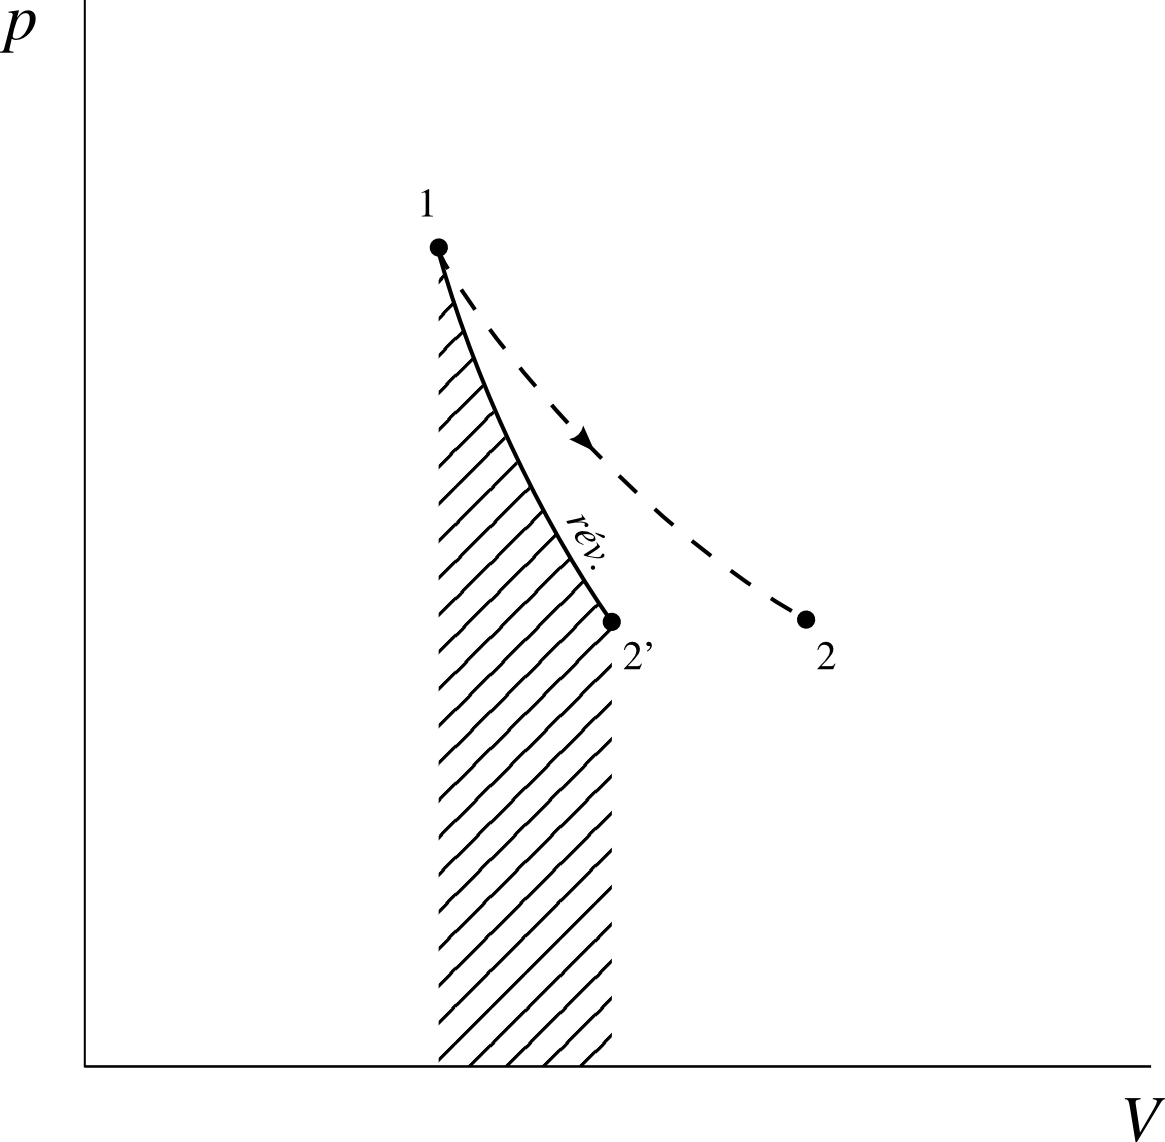
\includegraphics[width=8cm]{images/pv_reversible_irreversible.png}
			\end{center}
			\supercaption{Évolution du volume lors de détentes adiabatiques.
		L’augmentation du volume est calculable par l’intégration $\int \diff W / p$ le long d’un parcours réversible ($1 \to 2'$), mais pas le long d’un parcours irréversible ($1 \to 2$).}{schéma \cczero \oc}
			\label{fig_pv_reversible_irreversible}
		\end{figure}

		On peut voir que l’entropie est définie de façon similaire, c’est-à-dire comme étant la variable $S$ qui lors d’un transfert de chaleur réversible nous permet de lier la chaleur à la température avec la relation~\ref{eq_variation_franche_entropie} :
			\begin{equation*}
				\Delta S = \int_\A^\B \left( \frac{\diff Q}{T} \right)_\text{rév.}
			\end{equation*}
			\begin{equationterms}
				\item où l’indice \textit{rév.} spécifie que l’intégration se fait le long d’un chemin réversible.
			\end{equationterms}

		Nous avons alors
			\begin{IEEEeqnarray}{rCl}
				Q_\fromatob	& = & \int_\A^\B \left( T \diff S \right)_\text{rév.} \label{eq_q_tds_maj}\\
				q_\fromatob & = & \int_\A^\B \left( T \diff s \right)_\text{rév.} \label{eq_q_tds_min}
			\end{IEEEeqnarray}
			\begin{equationterms}
				\item pour toute évolution,
				\item où l’indice \textit{rév.} spécifie que l’intégration se fait le long d’un chemin réversible.
			\end{equationterms}

		Alors, nous allons pouvoir représenter les évolutions sur un \vocab{diagramme température-entropie}. L’aire sous la courbe d’une évolution représentera la chaleur transmise si l’évolution est réversible, mais pas si elle est irréversible, comme montré en \cref{fig_ts_reversible_irreversible}.

		\begin{figure}
			\begin{center}
				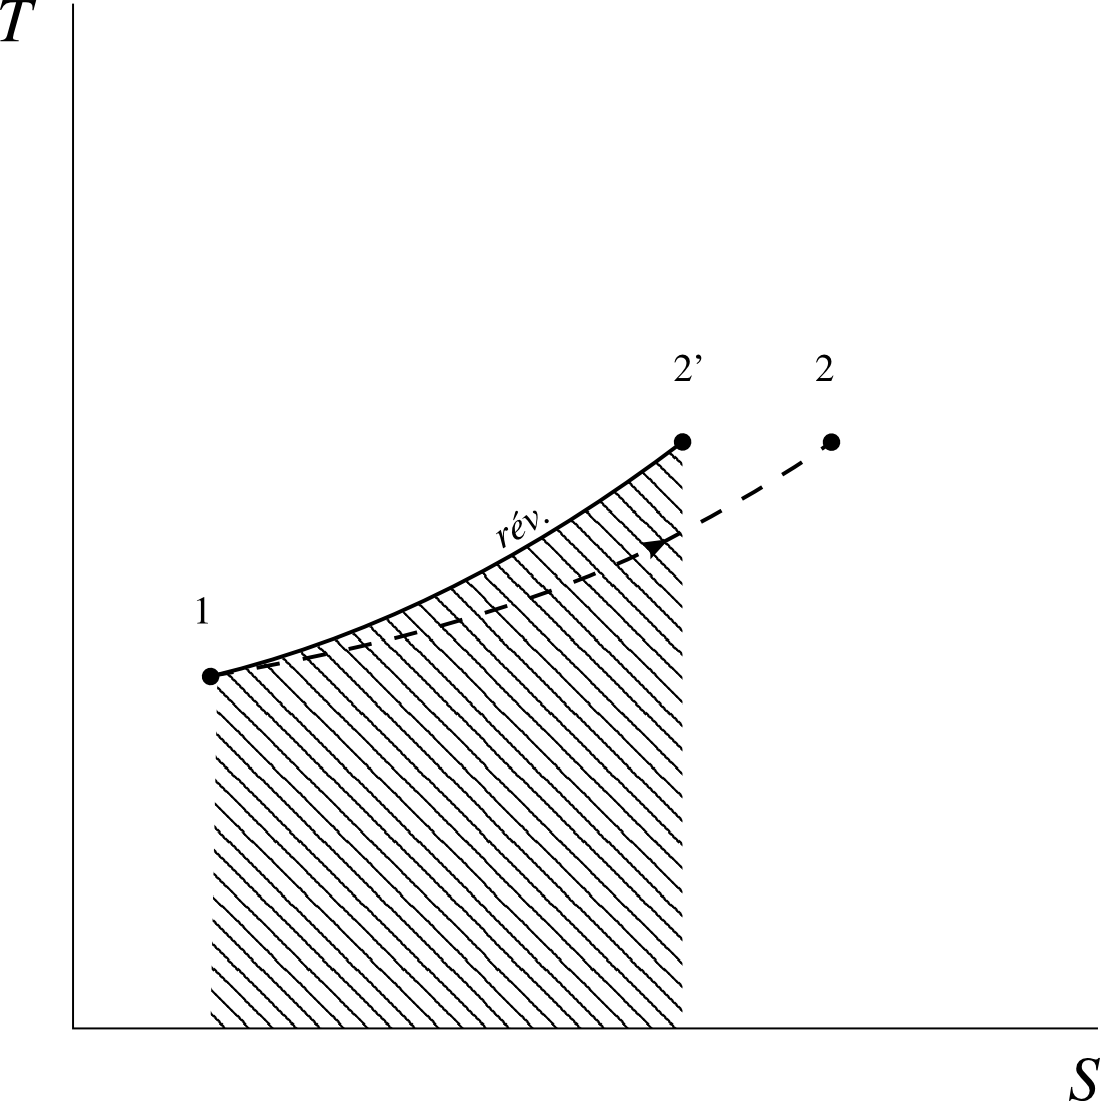
\includegraphics[width=8cm]{images/ts_reversible_irreversible.png}
			\end{center}
			\supercaption{Diagramme température-entropie. Lors d’une transformation réversible, l’aire sous la courbe d’un diagramme $T-S$ représente la chaleur transmise~$Q_{1 \to 2'}$ ; mais pas lorsqu’elle est irréversible.}{schéma \cczero \oc}
			\label{fig_ts_reversible_irreversible}
		\end{figure}

	
	\subsection{Les diagrammes température-entropie}
	
		Après six chapitres de bons et loyaux services, nous rangeons le diagramme pression-volume sur l’étagère, car il est temps de mettre à profit notre nouvel outil : le diagramme température-entropie. Même s’il est un peu plus abstrait, le diagramme $T-s$ est très utile pour décrire ce qui se passe à l’intérieur des machines car il est facile à tracer et il nous permet de visualiser directement \emph{l’irréversibilité}, qui est toujours indésirable pour l’ingénieur/e. 

		Lorsque le fluide reçoit ou fournit du travail de façon adiabatique réversible, alors $\Delta s = \int \frac{\diff q}{T} = 0$ puisque l’évolution est réversible et que $\diff q = 0$. Une transformation adiabatique réversible se fait donc à entropie constante --\ elle est iso-entropique, ce que nous appelons \vocab{isentropique}. Nous la représenterons ainsi par un trajet vertical sur les diagrammes température-entropie (\cref{fig_ts_basics}).

		\begin{figure}
			\begin{center}
				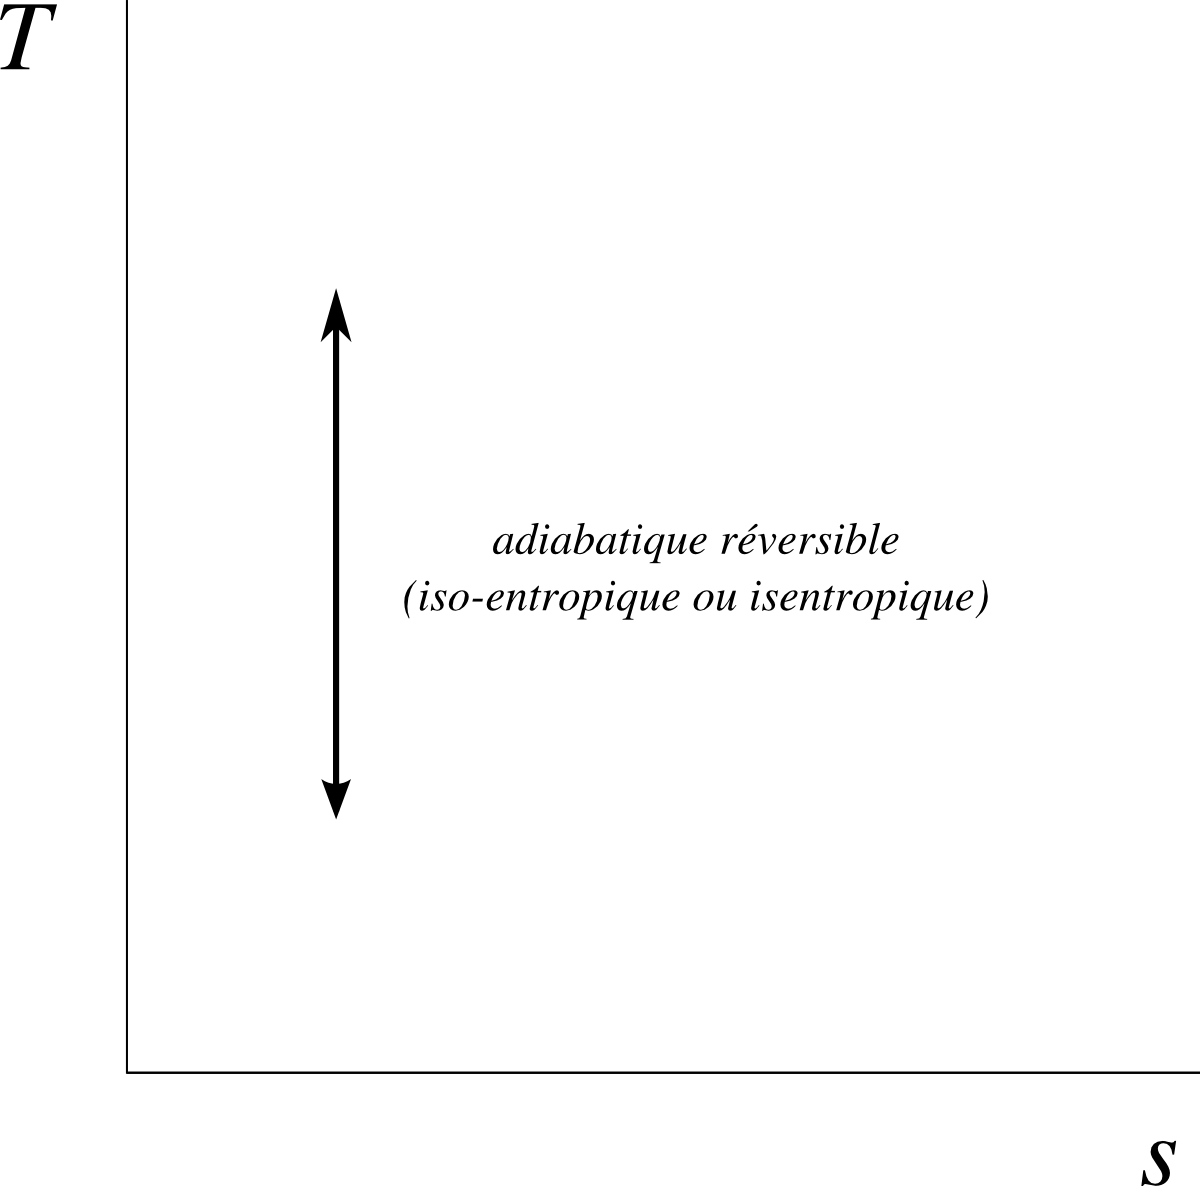
\includegraphics[width=0.47\textwidth]{images/ts_basics_1.png}
				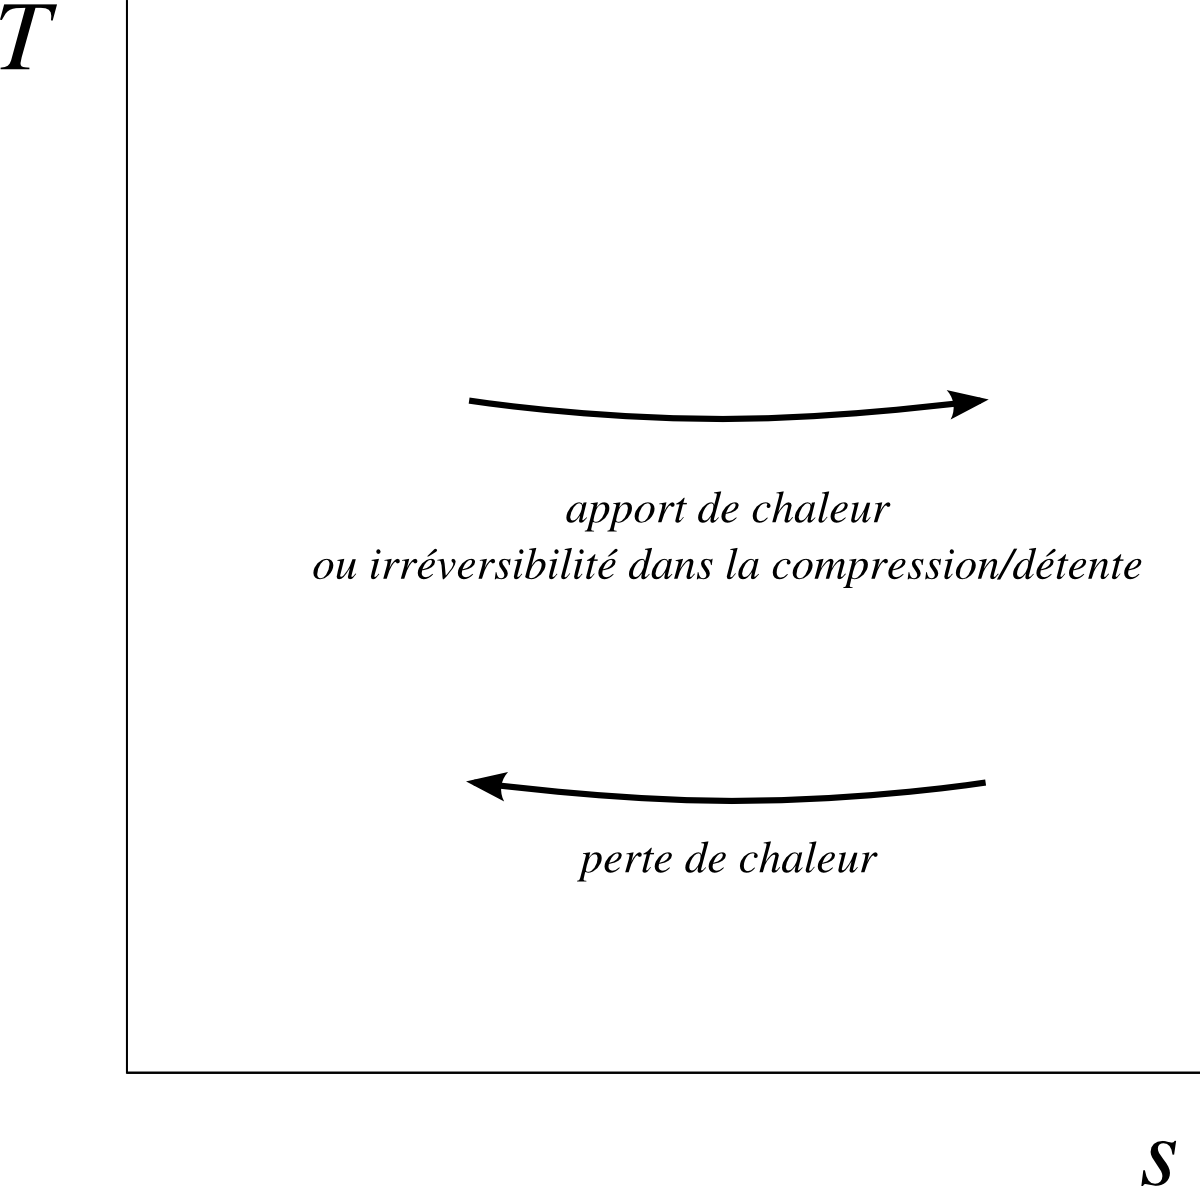
\includegraphics[width=0.47\textwidth]{images/ts_basics_2.png}
			\end{center}
			\supercaption{Évolutions élémentaires sur les diagrammes température-entropie.}{schéma \cczero \oc}
			\label{fig_ts_basics}
		\end{figure}

		Les transferts de chaleur, quant à eux, provoquent une variation de l’entropie du système (positive lorsque la chaleur est reçue, et négative lorsqu’elle est perdue). Sur les diagrammes $T-s$, nous nous déplacerons de gauche à droite lors des réceptions de chaleur ou bien lorsqu’il y a irréversibilité dans une compression ou une détente.

		Lorsque le système perd de la chaleur, son entropie décroît et nous nous déplacerons de droite à gauche sur les diagrammes $T-s$ (\cref{fig_ts_basics}).

		\clearfloats
		Notons aussi que, tout comme pour le volume, lorsqu’un fluide parcourt un cycle complet, il peut voir son entropie diminuer à une température plus faible qu’elle n’avait augmenté.
		%fin de phrase pas claire ici : "elle" c'est l'entropie (je suppose) ou la température ? En revanche c'est la température qui est "plus faible" mais qu'est-ce qui "avait augmenté" avant : la température, l'entropie... ? Je suggère de développer plus clairement le sens quitte à faire deux phrases distinctes.
		%tentative : Notons aussi que, tout comme pour le volume, lorsqu’un fluide parcourt un cycle complet, son entropie peut diminuer à une température inférieure à celle de sa phase d'augmentation (disclaimer : je ne sais pas de quoi je parle :) )
		%tentative2 : Notons aussi que lorsqu’un fluide parcourt un cycle complet, la température de diminution de l'entropie peut être inférieure à la température de son d'augmentation. Il en va de même pour le volume.
		Le transfert net de chaleur est alors négatif : le fluide a \emph{absorbé} de la chaleur qui aura été transformée en travail. En suivant le circuit inverse, le fluide sera source de chaleur : c’est le principe du réfrigérateur (\S\ref{ch_principe_fonctionnement_réfrigérateur}).
		
		Lorsque les évolutions sont réversibles, cette chaleur nette est représentée par l’aire enclose par le trajet sur un diagramme température-entropie (\cref{fig_ts_cycle}).

		\begin{figure}
			\begin{center}
				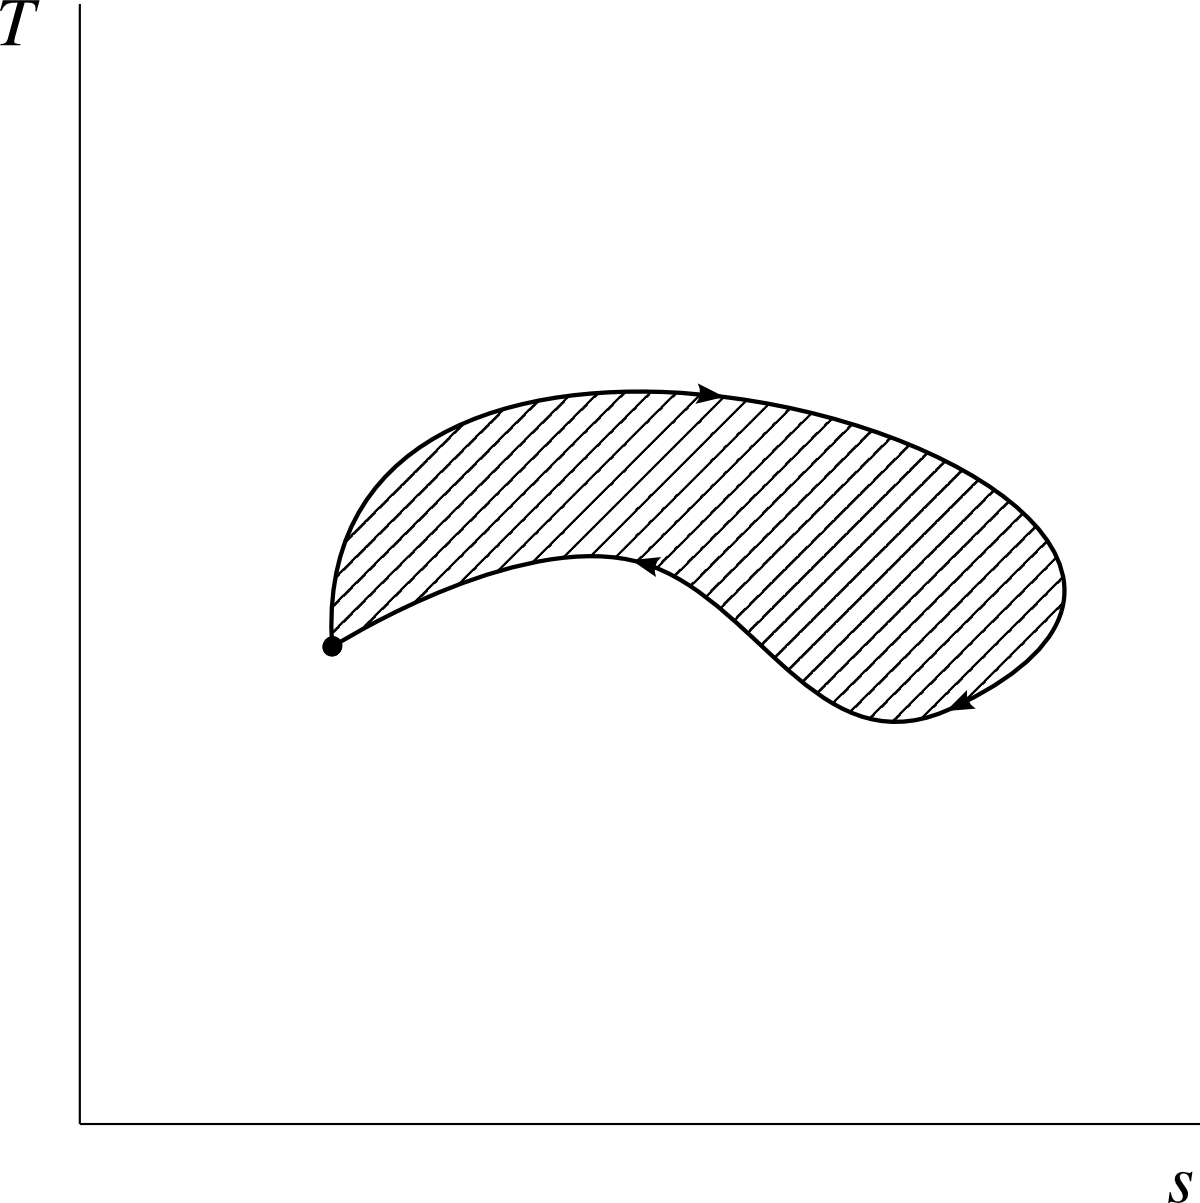
\includegraphics[width=8cm]{images/ts_cycle.png}
			\end{center}
			\supercaption{Cycle thermodynamique au cours duquel de la chaleur a été absorbée, et donc transformée en travail. Lorsque le trajet est effectué dans le sens inverse, de la chaleur est rejetée (et du travail absorbé) par le fluide.}{schéma \cczero \oc}
			\label{fig_ts_cycle}
		\end{figure}

		\clearfloats
		Enfin, nous notons avec joie que le cycle de Carnot, constitué de deux phases isothermes ($T = \text{cste}$) séparées par deux phases isentropiques ($s = \text{cste}$), gagne beaucoup à être représenté sur un diagramme température-entropie, comme montré en \cref{fig_ts_carnot}.

		\begin{figure}[htb]%handmade
			\begin{center}
				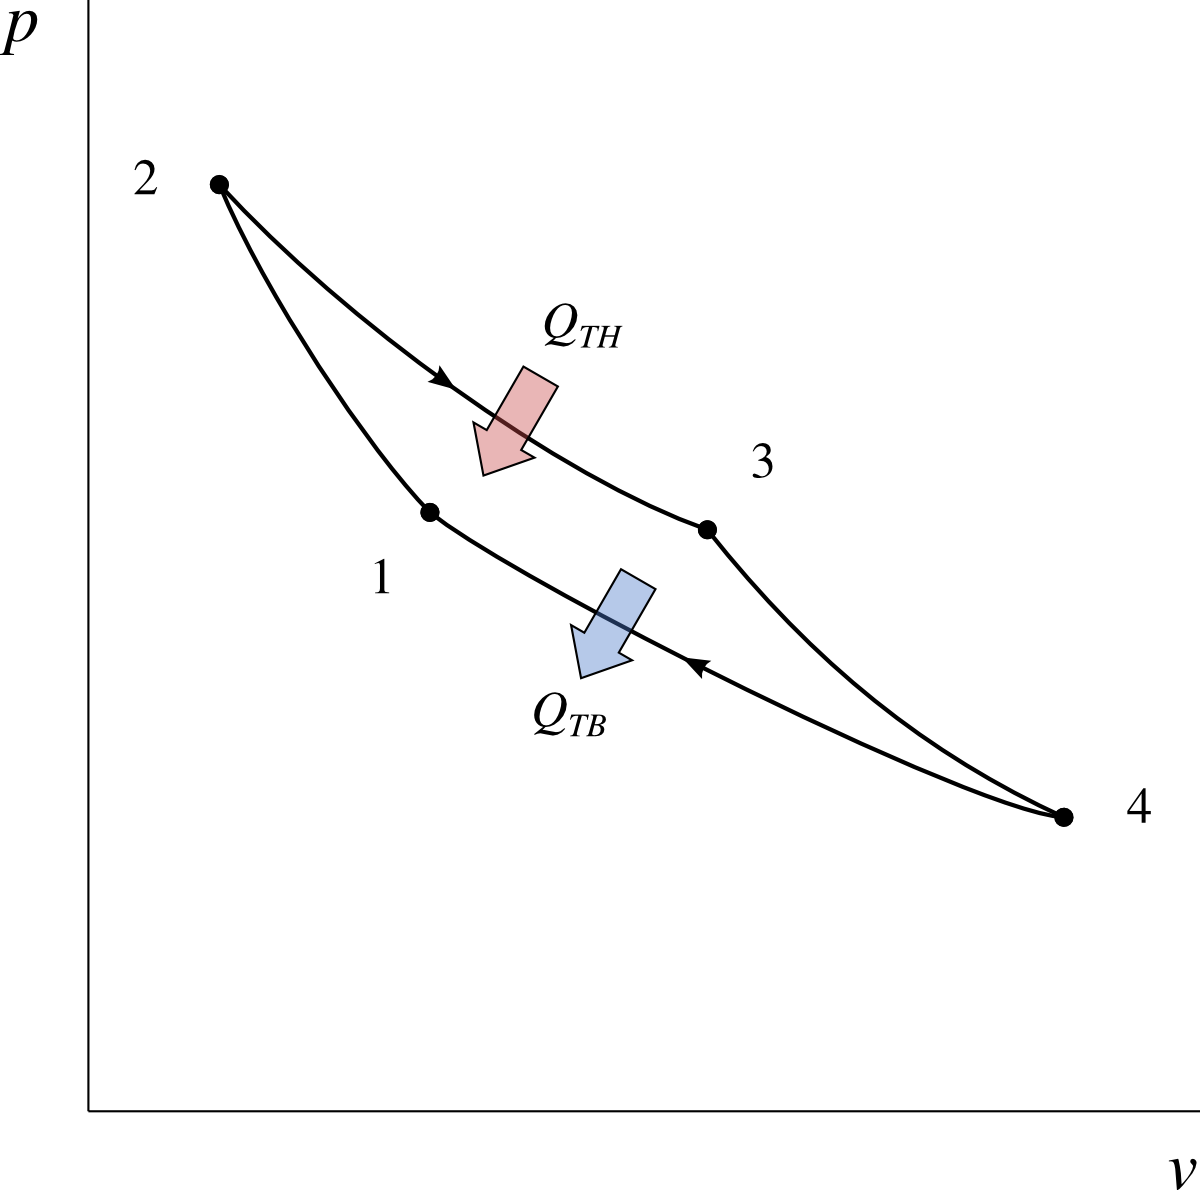
\includegraphics[width=0.49\textwidth]{images/pv_carnot_gp.png}
				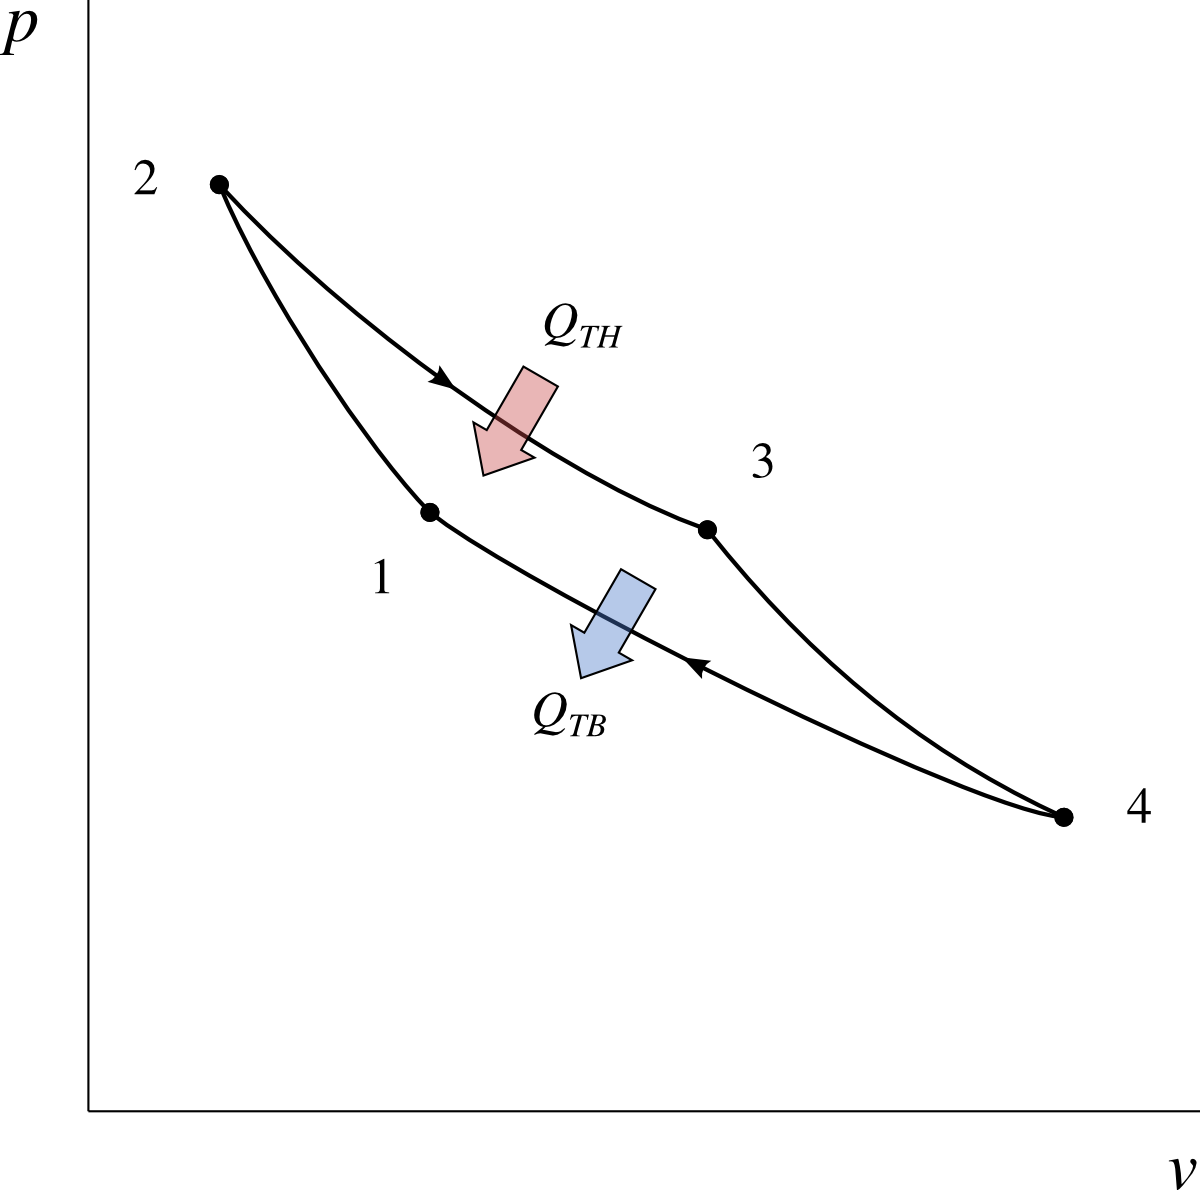
\includegraphics[width=0.49\textwidth]{images/pv_carnot_lv.png}
				\vspace{1cm}
				
				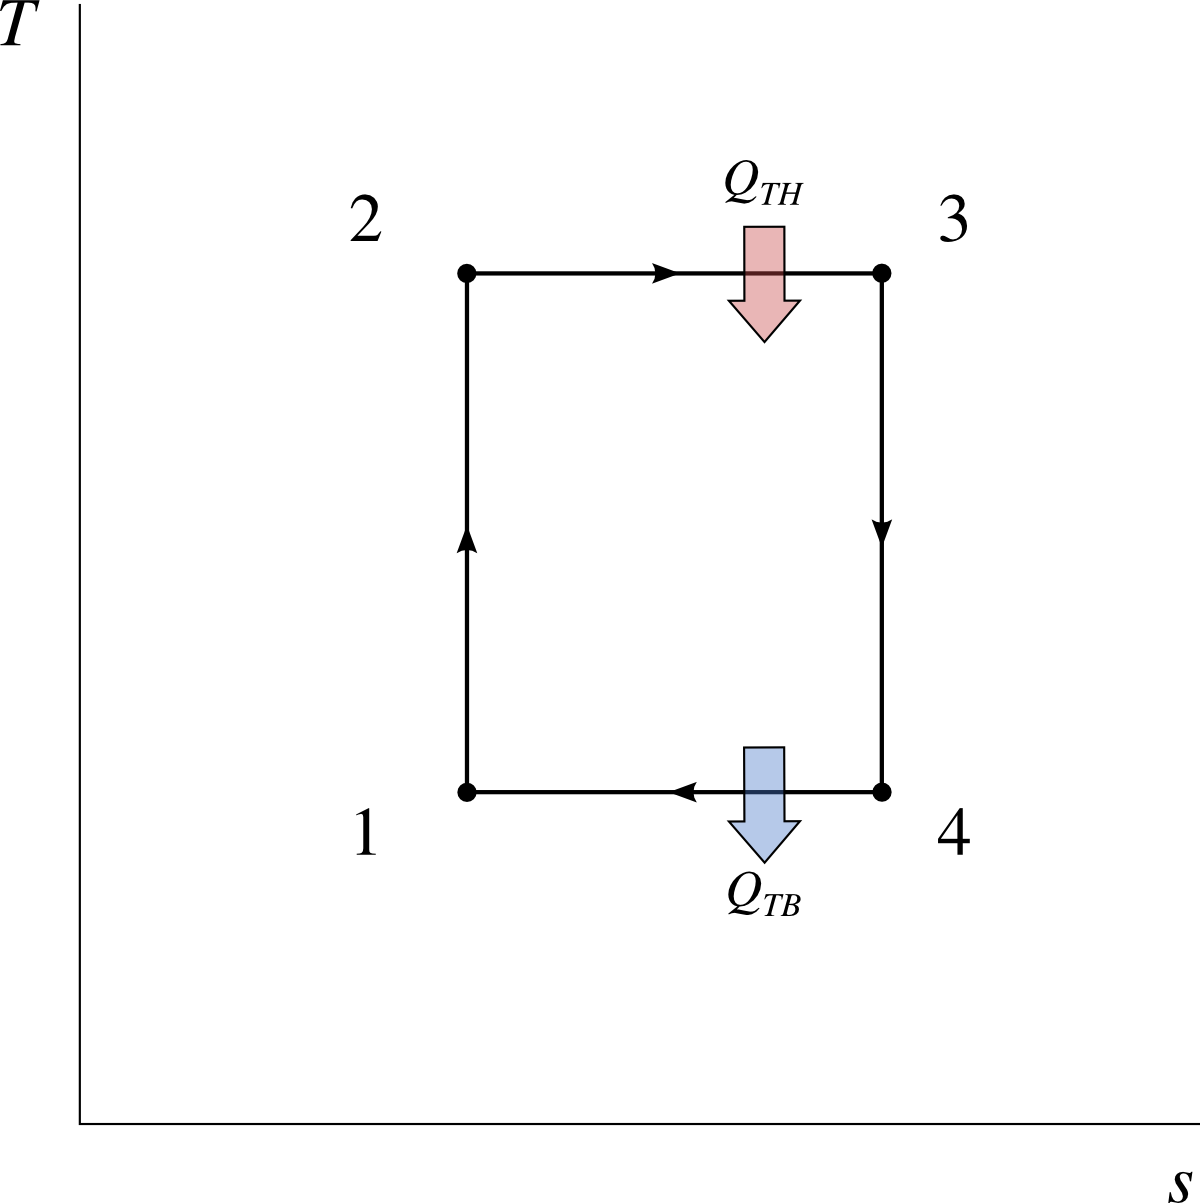
\includegraphics[width=8cm]{images/ts_carnot.png}
			\end{center}
			\supercaption{Cycle moteur de Carnot, sur un diagramme $p-v$ pour un gaz parfait (gauche), sur un diagramme $p-v$ pour un liquide-vapeur (droite), et sur un diagramme $T-s$ (bas). Quel que soit le fluide utilisé, le diagramme température-entropie reste le même.}{schéma \cczero \oc}
			\label{fig_ts_carnot}
		\end{figure}

	
	\subsection{Variations d’entropie d’un gaz parfait}
	\label{ch_delta_s_gaz_parfaits}
	
		À partir de maintenant, nous souhaitons pouvoir quantifier la variation d’entropie des fluides pour n’importe quelle évolution arbitraire. Dans le cas d’un gaz parfait, cette quantification est en fait étonnamment simple. 
	
		Pour n’importe quelle évolution d’une quantité fixe de fluide, nous avons (\ref{eq_premier_principe_sf_min}) :
			\begin{equation*}
				q_{1\to2} + w_{1\to2} = \Delta u
			\end{equation*}
		
		Si l’on imagine un chemin réversible entre 1 et 2, nous pouvons y quantifier $q_{1\to2} = -\int_1^2 T \diff s$ (\ref{eq_q_tds_min}) et $w_{1\to2} = -\int_1^2 p \diff v$ (\ref{eq_travail_pdv}), et nous pouvons donc écrire :
			\begin{IEEEeqnarray}{rCl}
				\int_1^2 T \diff s - \int_1^2 p \diff v 	& = & \Delta u \nonumber\\
				T \diff s - p \diff v 							& = & \diff u \nonumber\\
				\diff s 												& = & \frac{\diff u}{T} + \frac{p}{T} \diff v \label{eq_delta_s_u_p_v_t}
			\end{IEEEeqnarray}
			\begin{equationterms}
				\item le long de toute évolution réversible\footnote{Cette \cref{eq_delta_s_u_p_v_t} est même vraie pour toute évolution, mais cette généralisation est plus simple à aborder après les équations~\ref{eq_delta_s_gp_v} et~\ref{eq_delta_s_gp_p}.}\nolinebreak.
			\end{equationterms}
			
		Or, si nous utilisons un gaz parfait, nous avons $u = c_v T$ (\ref{eq_principe_de_joule})	et $\frac{p}{T} = \frac{R}{v}$ (\ref{eq_pv=RT}), ainsi :
			\begin{IEEEeqnarray}{rCl}
				\diff s 	& = & \frac{c_v \diff T}{T} + \frac{R}{v} \diff v \nonumber\\
							& = & c_v\frac{\diff T}{T} + R \frac{\diff v}{v} \nonumber\\
				\Delta s	= s_2 - s_1 & = & c_v \ln \frac{T_2}{T_1} + R \ln \frac{v_2}{v_1} \label{eq_delta_s_gp_v}\\
				\Delta s	= s_2 - s_1 & = & c_p \ln \frac{T_2}{T_1} - R \ln \frac{p_2}{p_1} \label{eq_delta_s_gp_p}
			\end{IEEEeqnarray}
			\begin{equationterms}
				\item pour un gaz parfait,
				\item pour toute évolution de 1 à 2, réversible ou non.
			\end{equationterms}

			\thermoquotebegin{O}	
				Dans l’expression obtenue, la différence $S - S_0$ est de nouveau entièrement déterminée si les états de départ et d’arrivée sont connus, et nous ne devons prêter attention à la manière dont s’est déroulé le passage de l’un vers l’autre que lorsque nous formons l’intégrale $\int \frac{\diff Q}{T}$.
			\thermoquoteend{Rudolf Clausius, 1865~\cite{clausius1865,clausius1867en,clausius1868fr2}}{}

		Cette équation est intéressante parce qu’elle nous indique que la variation d’entropie $\Delta s$ pendant une évolution de $1$ à $2$ ne dépend que des états initial et final. Même si nous avons commencé cette démonstration le long d’une évolution réversible nous obtenons une expression~\ref{eq_delta_s_gp_v} dans laquelle le chemin utilisé n’apparaît~pas. 
		
		Il est donc possible de calculer facilement la variation d’entropie d’un gaz parfait si l’on connaît ses autres propriétés. Contrairement à l’énergie interne $u$ qui ne dépend que de la température, l’entropie $s$ dépend aussi de la pression du gaz.

		Dans le cas où la pression ou le volume spécifique sont maintenus constants, il est facile de montrer que ces équations~\ref{eq_delta_s_gp_v} et~\ref{eq_delta_s_gp_p} deviennent respectivement :
			\begin{IEEEeqnarray}{rCl}
				\Delta s_{v_\text{cst.}} 		& = & c_v \ln \frac{T_2}{T_1} 	\label{eq_delta_s_gp_vcst} \\
				\Delta s_{p_\text{cste}} 		& = & c_p \ln \frac{T_2}{T_1} 	\label{eq_delta_s_gp_pcste}
			\end{IEEEeqnarray}
			\begin{equationterms}
				\item pour un gaz parfait,
				\item pour toute évolution à volume constant ou respectivement à pression constante.
			\end{equationterms}

		Ces deux équations~\ref{eq_delta_s_gp_vcst} et~\ref{eq_delta_s_gp_pcste} nous permettent de tracer des courbes isochores (à volume constant) et isobares (à pression constante) pour un gaz parfait sur un diagramme $T-s$, comme montré en \cref{fig_ts_gp_isobares_isochores}.

		\begin{figure}
			\begin{center}
				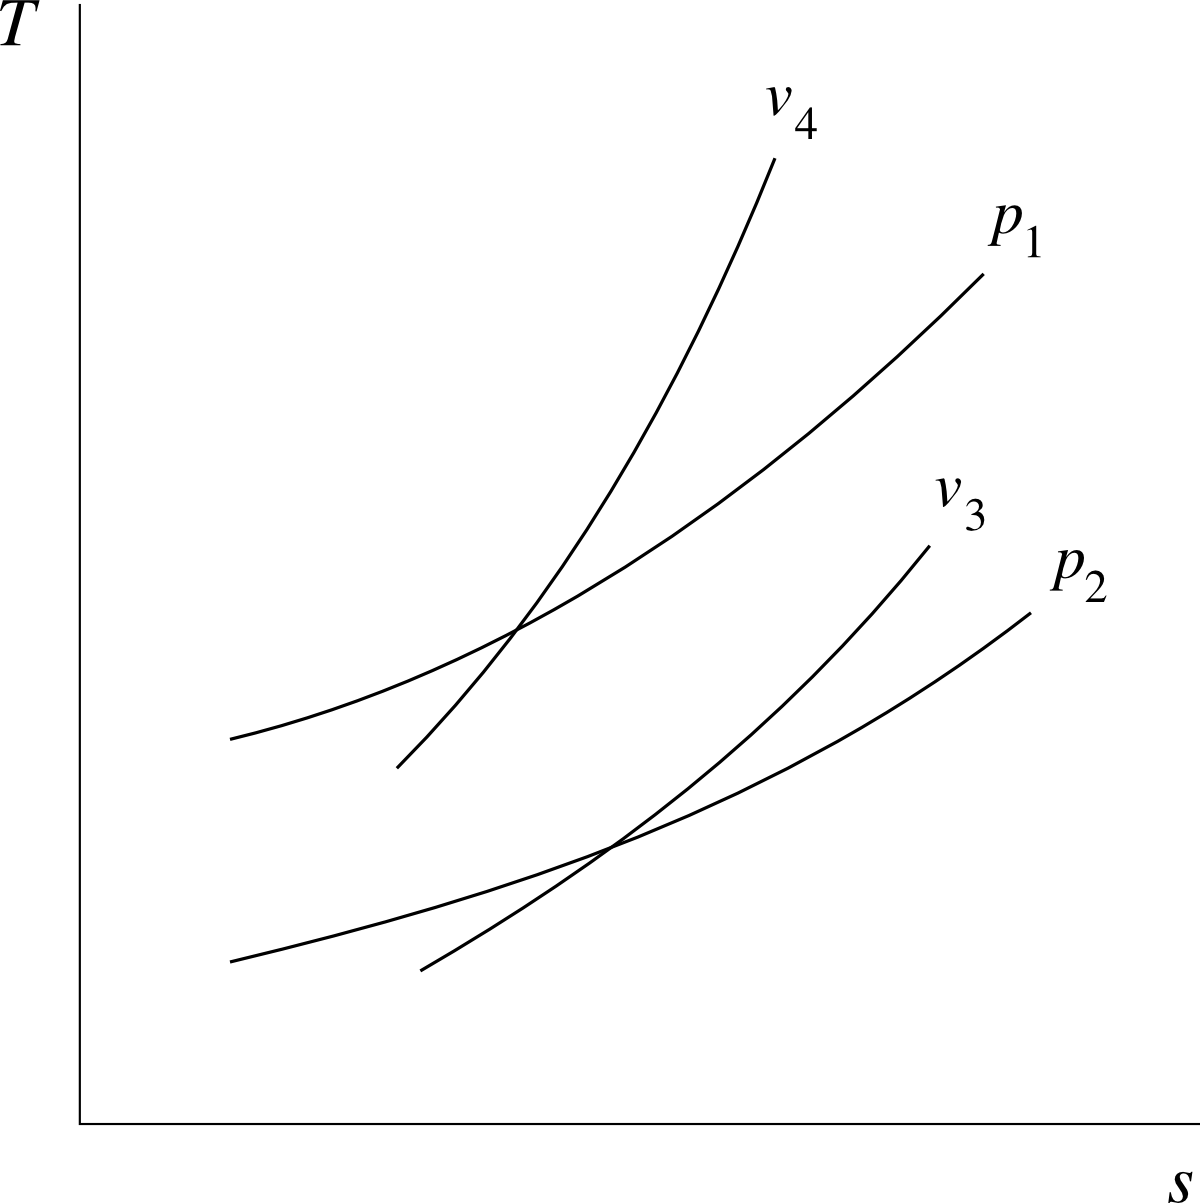
\includegraphics[width=\didacticpvdiagramwidth]{images/ts_gp_isobares_isochores.png}
			\end{center}
			\supercaption{Courbes isobares et isochores sur un diagramme $T-s$, pour un gaz parfait. Ici $p_1>p_2$ et $v_3>v_4$.}{schéma \cczero \oc}
			\label{fig_ts_gp_isobares_isochores}
		\end{figure}

		\clearfloats
		\begin{anexample}
			Quelle est la variation d’entropie spécifique d’une masse de~\SI{2}{\kilogram} d’air, lorsqu’elle est chauffée à pression constante de~\SI{2}{\bar}, depuis \SI{10}{\degreeCelsius} jusqu’à~\SI{100}{\degreeCelsius} ?
			
				\begin{answer}
					L’évolution peut être représentée de façon qualitative sur un diagramme température-entropie ainsi :
						\begin{center}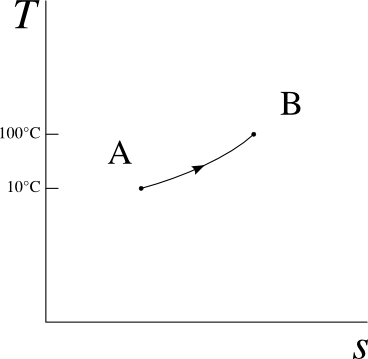
\includegraphics[width=4cm]{images/exe_ts_1.png}\end{center}
					Pour calculer $\Delta S$ nous partons de l’\cref{eq_delta_s_gp_p}, $\Delta s = c_p \ln \frac{T_\B}{T_\A} - R \ln \frac{p_\B}{p_\A}$ et ici $p_\B=p_\A$. Nous avons donc $\Delta s = c_p \ln \frac{T_\B}{T_\A} = \num{1005} \ln \frac{100+273,15}{10+273,15} =  \SI{+277,4}{\joule\per\kelvin\per\kilogram}$. \\L’entropie varie donc de $\Delta S = m \ \Delta s = 2 \times 277,4 = \SI{+554,8}{\joule\per\kelvin}$. 
				\begin{remark}Peu nous importe que l’évolution soit réversible ou non : il nous suffit de connaître les états initial et final.\end{remark}
				\begin{remark}Nous écrivons bien que «~l’entropie de l’air augmente~» et non pas qu’«~on lui donne de l’entropie~» (\S\ref{ch_entropie_propriete}).\end{remark}\end{answer}
		\end{anexample}


		\begin{anexample}
			De combien varie l’entropie d’une masse d’air de~\SI{0,5}{\kilogram} refroidie lentement à température constante depuis \SI{1}{\bar} et~\SI{50}{\degreeCelsius} jusqu’à~\SI{5}{\bar} ? Combien faut-il lui prendre de chaleur pour cela ?
			
				\begin{answer}
					L’évolution peut être représentée de façon qualitative sur un diagramme $T-s$ ainsi :
						\begin{center}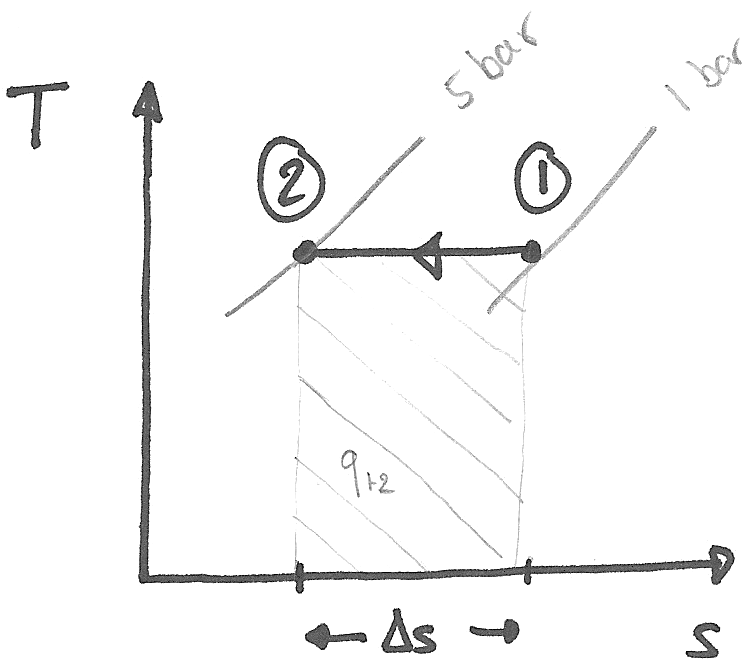
\includegraphics[width=4cm]{images/exe_ts_2.png}\end{center}
					Pour quantifier $\Delta S$ nous partons de l’\cref{eq_delta_s_gp_p}, $\Delta s = c_p \ln \frac{T_B}{T_A} - R \ln \frac{p_B}{p_A}$ et ici $T_B=T_A$. Nous avons donc $\Delta s = -R \ln \frac{p_B}{p_A} = \num{287} \ln \frac{5}{1} =  \SI{-461,9}{\joule\per\kelvin\per\kilogram}$. \\L’entropie varie donc de $\Delta S = m \ \Delta s = \num{0,5} \times \num{-461,9} = \SI{-231}{\joule\per\kelvin}$. 
					
					Comme l’évolution est réversible, la chaleur prélevée s’obtient avec l’\cref{eq_q_tds_maj} : $Q_{\fromatob} = \int_\A^\B T \diff S = T_\text{cste} \int_\A^\B \diff S = T_\text{cste} \Delta S = (50+273,15) \times \num{-231} = \SI{-74,6}{\kilo\joule}$. 
				
				\begin{remark}Nous savions déjà quantifier $Q_{\fromatob}$ sans utiliser l’entropie, à l’aide des équations \ref{eq_gp_travail_isotherme_sf2} et \ref{eq_gp_chaleur_isotherme_sf}.\end{remark}\end{answer}
		\end{anexample}

		\begin{anexample}
			De combien varie la température d’une masse d’air détendue de façon adiabatique réversible depuis \SI{30}{\bar} et~\SI{600}{\kelvin} jusqu’à~\SI{1}{\bar} ?
			
				\begin{answer}
					L’évolution peut être représentée de façon qualitative sur un diagramme $T-s$ ainsi :
						\begin{center}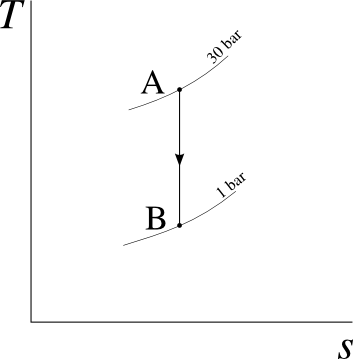
\includegraphics[width=4cm]{images/exe_ts_3.png}\end{center}
					Pour quantifier $\Delta S$ nous partons encore de l’\cref{eq_delta_s_gp_p} : $\Delta s = c_p \ln \frac{T_\B}{T_\A} - R \ln \frac{p_\B}{p_\A}$ et ici $\Delta s = 0$ :\vspace{-1cm}
					
						\begin{IEEEeqnarray*}{rCl}
							0 											& = & c_p \ln \frac{T_\B}{T_\A} - R \ln \frac{p_\B}{p_\A} \\
							\ln \frac{T_\B}{T_\A}				& = & \frac{R}{c_p} \ln \frac{p_\B}{p_\A} \\
							\left(\frac{T_\B}{T_\A}\right)	& = & \left(\frac{p_\B}{p_\A}\right)^{\frac{R}{c_p}} = \left(\frac{p_\B}{p_\A}\right)^{\frac{\gamma-1}{\gamma}}
						\end{IEEEeqnarray*}
				
					Nous reconnaissons ainsi l’\cref{eq_isentropique_horrible2} que nous savons déjà appliquer : $T_\B = 600 \times \frac{1}{30}^{\frac{0,4}{1,4}} =  \SI{227}{\kelvin} $, soit environ \SI{-46}{\degreeCelsius}.
				
				\begin{remark}L’utilisation du raisonnement «~adiabatique réversible = isentropique~» ne nous a, en vérité, rien apporté que nous ne savions déjà ici, car le modèle du gaz parfait est déjà extrêmement simple et puissant. Ce ne sera pas le cas avec les liquides/vapeurs.\end{remark}\end{answer}
		\end{anexample}


	\subsection{Variations d’entropie d’un liquide/vapeur}
	
		Pour un liquide/vapeur, les variations ne peuvent pas être calculées car il n’existe pas de modèle mathématique simple pour modéliser la température en fonction des autres propriétés. La courbe de saturation et le chemin d’une évolution à pression constante sont représentés en \cref{fig_ts_lv} ; cette figure~ressemble très fortement au diagramme température-volume que nous avions tracé en \cref{fig_t-v_eau}.
		Pour quantifier les valeurs de $s$, nous allons procéder exactement comme avec l’énergie interne $u$ au \courscinqshort~: en les tabulant.

		\begin{figure}
			\begin{center}
				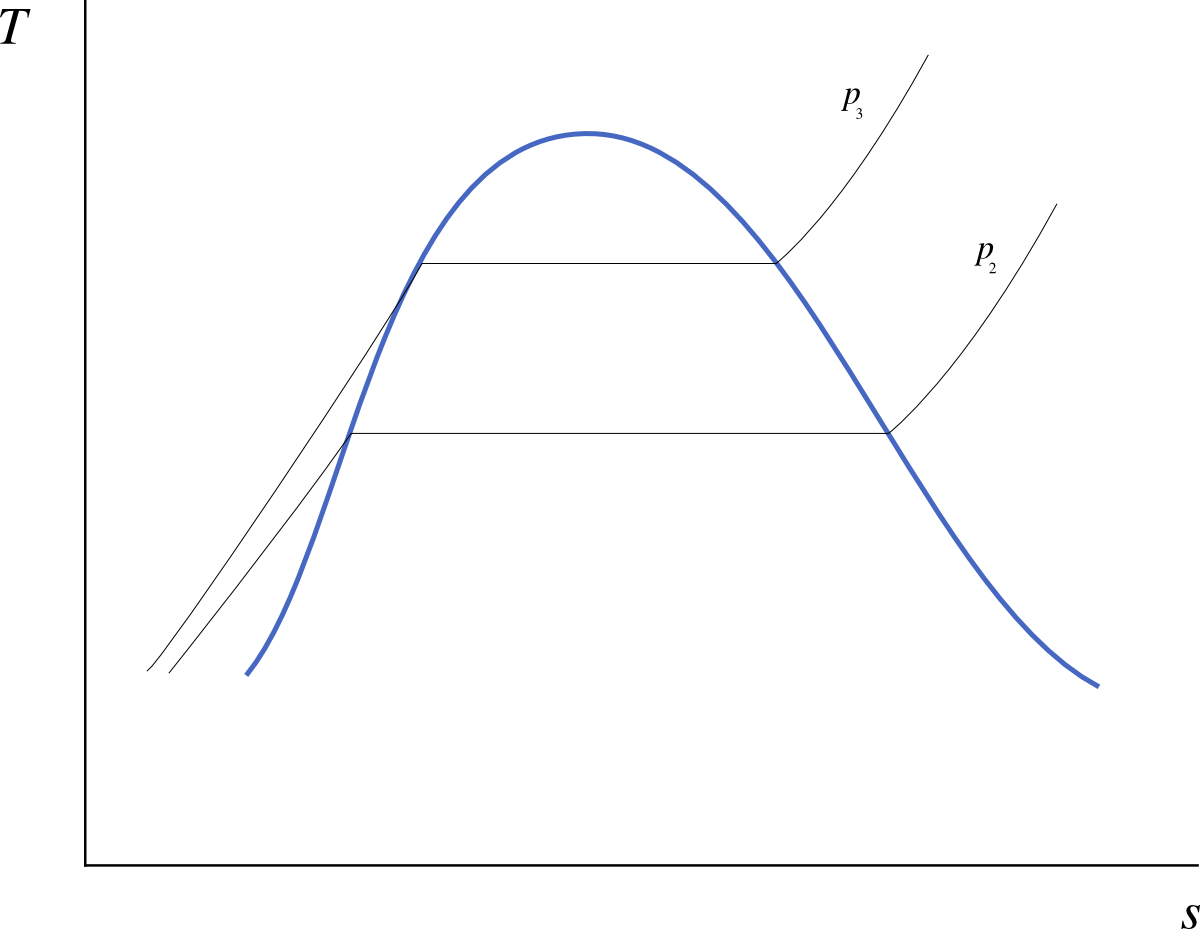
\includegraphics[width=\didacticpvdiagramwidth]{images/ts_lv.png}
			\end{center}
			\supercaption{Diagramme température-entropie d’un liquide/vapeur. Cette figure est très similaire à la \cref{fig_t-v_eau}.}{schéma \cczero \oc}
			\label{fig_ts_lv}
		\end{figure}
		
		En dehors des phases de mélange (c’est-à-dire lorsque l’eau est à l’état de liquide comprimé ou de vapeur sèche) les valeurs de l’entropie\footnote{En réalité, toutes les valeurs tabulées de l’entropie sont relatives à un point de référence pour lequel la valeur de $s$ est arbitrairement posée à~\SI{0}{\joule\per\kelvin\per\kilogram} ; dans notre cas, c’est le point triple de l’eau. Cela n’a pas d’importance dans nos calculs puisque seules les variations de l’entropie nous intéressent.} peuvent simplement être lues en dernière colonne dans l’abaque~n°1, dont un extrait est répété dans le \cref{tab_abaque1extraitbis}.
		
		\begin{table}
		\begin{center}
		\begin{footnotesize}
		\begin{tabular}{
		|S[table-format = 4.0]|%				T
		S[table-format = 2.6]% 		v
		S[table-format = 4.1]%			u
		S[table-format = 4.1]%		h
		S[table-format = 2.4]|%	s
		}

 		\hline
		%\addlinespace[10pt]
		 &&&&\\
		\multicolumn{1}{|@{}c@{}|}{{\scriptsize °C}}	% Using SIunit screws the table up here for some reason
		&\multicolumn{1}{@{}c@{}}{{\small\si[per-mode = fraction]{\metre\cubed\per\kilogram}}}%
		&\multicolumn{1}{@{}c@{}}{{\small\si[per-mode = fraction]{\kilo\joule\per\kilogram}}}%
		&\multicolumn{1}{@{}c@{}}{{\small\si[per-mode = fraction]{\kilo\joule\per\kilogram}}}%
		&\multicolumn{1}{@{}c@{}|}{{\small\si[per-mode = fraction]{\kilo\joule\per\kilogram\per\kelvin}}}\\%

		%\addlinespace[10pt]
		 &&&&\\
		{$T$}	&$v$	&$u$	&$h$	&$s$\\
		\hline
 		
		&\multicolumn{4}{c|}{$p = \SI{1,6}{\mega\pascal}$}\\
		&\multicolumn{4}{c|}{($T_\text{sat} = \SI{201,37}{\degreeCelsius}$)}\\
		
		10		&0,001		&42		&43,6		&0,1509\\
		20		&0,001001	&83,8		&85,4		&0,2962\\
		50		&0,001011	&209,1	&210,7	&0,7031\\
		100	&0,001043	&418,6	&420,3	&1,306\\
		200	&0,001156	&850,4	&852,3	&2,3305\\	\cdashline{2-5}[.8pt/2pt]
		300	&0,15866	&2781,5	&3035,4	&6,8863\\
		500	&0,22029	&3120,1	&3472,6	&7,5409\\
		600	&0,24999	&3293,9	&3693,9	&7,81\\
		700	&0,2794	&3473,5	&3920,5	&8,0557\\
		800	&0,30865	&3659,5	&4153,3	&8,2834\\
		900	&0,3378	&3852,1	&4392,6	&8,4965\\
		1000	&0,36687	&4051,2	&4638,2	&8,6974\\
		1100	&0,39589	&4256,6	&4890		&8,8878\\
		1200	&0,42487	&4467,9	&5147,7	&9,0689\\
		1500	&0,51169	&5133,7	&5952,4	&9,5656\\
		2000	&0,65615	&6326,8	&7376,6	&10,272\\
		\hline

 		\end{tabular}\end{footnotesize}\end{center}
 		\caption{Extrait de l’abaque~n°1. L’entropie peut être lue en dernière colonne et ses valeurs interpolées comme les autres propriétés.}
 		\label{tab_abaque1extraitbis}
 		\end{table}

	
		À l’intérieur de la courbe de saturation les valeurs de $s$ s’interpolent entre celles de $s_L$ (liquide saturé) et $s_V$ (vapeur saturée) à l’aide de la notion de \emph{titre}, exactement comme avec l’\cref{eq_titre_energie_interne} :
		\begin{equation}
			s_x = s_L + x \ s_{LV}
			\label{eq_titre_entropie}
		\end{equation}
	
		\clearfloats
		\begin{anexample}
			Quelle est la variation de l’entropie de l’eau lorsqu’elle part d’un état à~\SI{240}{\degreeCelsius} et~\SI{6}{\bar}, pour arriver à~\SI{130}{\degreeCelsius} avec une énergie interne de~\SI{1000}{\kilo\joule\per\kilogram} ?% surch → mélange liq/v
			
				\begin{answer}
					Un bref coup d’œil dans les abaques de vapeur nous permet de représenter l’évolution de façon qualitative sur un diagramme $T-s$ ainsi :
						\begin{center}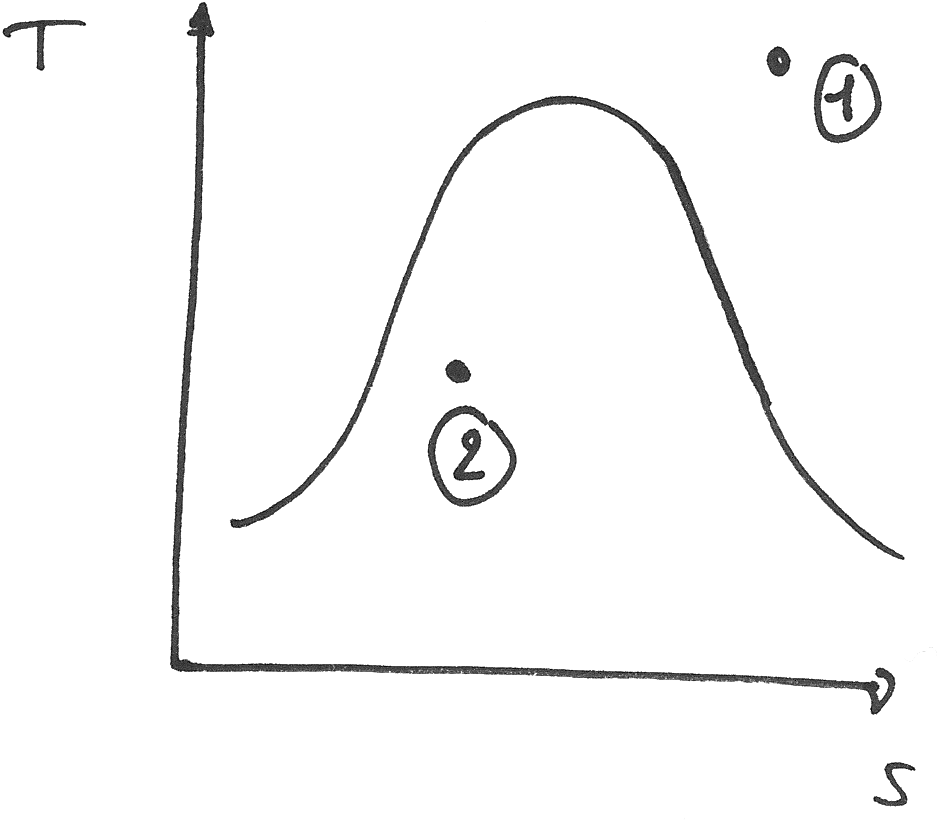
\includegraphics[width=4cm]{images/exe_ts_4.png}\end{center}
					Nous lisons $s_\A$ par interpolation dans l’abaque n°1 à~\SI{0,6}{\mega\pascal} entre \SI{200}{\degreeCelsius} et~\SI{300}{\degreeCelsius} : $s_\A= \num{6,9683} + \frac{40}{100}\times(\num{7,374}-\num{6,9683}) = \SI{7,1306}{\kilo\joule\per\kelvin\per\kilogram} $.\\
					À l’arrivée, l’eau est en mélange liquide-vapeur (puisque $u_\B<u_{V\SI{130}{\degreeCelsius}}$), nous lisons donc en abaque n°2 (\ref{eq_titre_energie_interne}) : $x_\B = \frac{u_\B - u_L}{u_{LV}} = \frac{\num{1000}-\num{546,1}}{\num{1993,5}}= \num{0,228} $ ; ainsi avec l’\cref{eq_titre_entropie} nous pouvons calculer l’entropie : $s_\B= s_L + x_\B \ s_{LV} = \num{1,6346}+ \num{0,228}\times\num{5,3918} = \SI{2,8623}{\kilo\joule\per\kelvin\per\kilogram}$.\\
					Nous voyons que l’entropie a diminué : $\Delta s = s_\B - s_\A = \SI{-4,268}{\kilo\joule\per\kelvin\per\kilogram} $.
				
				\begin{remark}Nous ne savons pas quelle transformation a eu lieu. Moins elle a été réversible, plus il aura fallu retirer de la chaleur à la vapeur pour l’amener de~A à~B.\end{remark}\end{answer}
		\end{anexample}

		
		\begin{anexample}
			On réchauffe lentement \SI{2}{\kilogram} d’eau liquide saturée à~\SI{300}{\degreeCelsius}, en maintenant sa température constante, jusqu’à ce que le volume atteigne \SI{2}{\metre\cubed}. Combien de chaleur faut-il apporter pour cela ?
			
				\begin{answer}
					Un bref coup d’œil dans les abaques de vapeur nous permet de représenter l’évolution de façon qualitative sur un diagramme $T-s$ ainsi :
						\begin{center}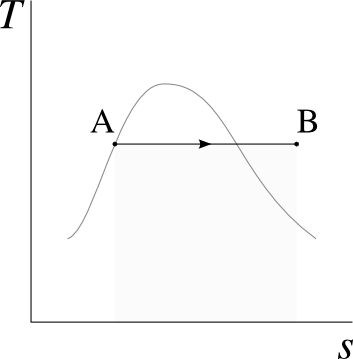
\includegraphics[width=4cm]{images/exe_ts_5.png}\end{center}
				Comme l’évolution est réversible nous allons pouvoir calculer $Q_{\fromatob}$ en intégrant le terme $T \diff s$ entre A et B. \\
				Nous lisons $s_\A$ dans l’abaque n°2 : $s_\A = s_{L\SI{300}{\degreeCelsius}} = \SI{3,2552}{\kilo\joule\per\kilogram}$.\\
				À l’arrivée le volume spécifique est $v_\B = \frac{V_\B}{m} = \frac{2}{2} = \SI{1}{\metre\cubed\per\kilogram} $ ; pour obtenir $s_\B$ il faut interpoler entre deux blocs de l’abaque n°1 (entre \SI{0,2}{\mega\pascal} et~\SI{0,4}{\mega\pascal} à~\SI{300}{\degreeCelsius}). 
				Nous posons $y \equiv \frac{v_\B - v_{\SI{300}{\degreeCelsius}~\&~\SI{0,2}{\mega\pascal}}}{v_{\SI{300}{\degreeCelsius}~\&~\SI{0,4}{\mega\pascal}} - v_{\SI{300}{\degreeCelsius}~\&~\SI{0,2}{\mega\pascal}}} = \frac{1 -\num{1,3162}}{\num{0,65489}-\num{1,3162}} = \num{0,4781} $
				et de façon correspondante, $s_\B = s_{\SI{300}{\degreeCelsius}~\&~\SI{0,2}{\mega\pascal}} + y (s_{\SI{300}{\degreeCelsius}~\&~\SI{0,4}{\mega\pascal}} - s_{\SI{300}{\degreeCelsius}~\&~\SI{0,2}{\mega\pascal}}) = \SI{7,8941} + \num{0,4781}(\num{7,5677}-\SI{7,8941}) = \SI{7,738}{\kilo\joule\per\kelvin\per\kilogram} $.
				
				Nous pouvons donc enfin calculer $q_{\fromatob}$ avec l’\cref{eq_q_tds_min} : $Q_{\fromatob} = 	\int_1^2 T \diff S = m \ T \ \Delta s = 2 \times (300+\num{273,15})\times(\num{7,738} - \num{3,2552}) = \SI{+5,139}{\kilo\joule} $.
				
				\begin{remark}Ce calcul un peu laborieux n’est pas nécessairement spectaculaire, mais il faut bien voir que sans l’utilisation de l’entropie, nous n’avions pas de moyen de quantifier $Q_{\fromatob}$ sans effectuer d’expérience.\end{remark}\end{answer}
		\end{anexample}
		
		
		\begin{anexample}
			Dans une turbine la vapeur est détendue de façon adiabatique réversible (isentropique). La vapeur entre à~\SI{40}{\bar} et~\SI{500}{\degreeCelsius} ; elle est détendue jusqu’à~\SI{0,5}{\bar}. Quelle est la puissance spécifique fournie ?
			
				\begin{answer}
					Un dernier coup d’œil dans les abaques de vapeur nous permet de représenter l’évolution de façon qualitative sur un diagramme $T-s$ ainsi :
						\begin{center}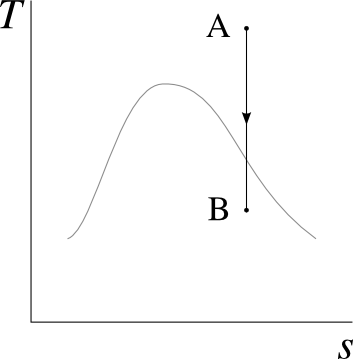
\includegraphics[width=4cm]{images/exe_ts_6.png}\end{center}
				Ici $q_{\fromatob} = 0$ car la turbine est adiabatique, et nous cherchons $w_{\fromatob} = \Delta h$. Il nous faut donc trouver un moyen de quantifier $h_\B$.
				
				En A nous lisons dans l’abaque n°1, à~\SI{4}{\mega\pascal} : $h_\A = \SI{3446}{\kilo\joule\per\kilogram}$ et $s_\A = \SI{7,0922}{\kilo\joule\per\kelvin\per\kilogram}$.
				
				En B nous savons que $s_\B = s_\A$ car l’évolution est isentropique ; cette information va nous permettre de calculer $h_\B$. Dans l’abaque n°2 à~\SI{0,05}{\mega\pascal}, avec l’\cref{eq_titre_entropie} nous obtenons $x_\B = \frac{s_\B - s_L}{s_{LV}} = \frac{\num{7,0922}-\num{1,0912}}{\num{6,5018}} = \num{0,923}$. Avec le titre nous pouvons simplement calculer l’enthalpie (\ref{eq_titre_enthalpie}) : $h_\B = h_L + x_\B \ h_{LV} = \num{340,5} + \num{0,923}\times\num{2304,7} = \SI{2467,7}{\kilo\joule\per\per\kilogram}$.
				
				La puissance spécifique de la turbine est donc de $w_{\fromatob} = \Delta h = \SI{-978,3}{\kilo\joule\per\kilogram}$.
				
				\begin{remark}Le calcul que nous venons de faire est extrêmement utile pour l’ingénieur/e. L’idée que l’entropie reste constante pendant une évolution adiabatique réversible nous permet --\ enfin!\ -- de prédire l’état d’un liquide-vapeur à la sortie d’un compresseur ou d’une turbine. Jusqu’à présent, nous pouvions le faire avec un gaz parfait (et les encombrantes relations de type $\frac{T_1}{T_2} = …$), mais pas pour un liquide/vapeur.\end{remark}\end{answer}
		\end{anexample}



\section{Prédire le sens des transformations}

	Nous voilà au concept central qui a ouvert les portes de la physique à la thermodynamique. À partir des quantifications des variations d’entropie, nous sommes capables de décrire le sens des transformations, c’est-à-dire de prouver par exemple qu’un état B vient \emph{après} un état A. 

	\subsection{Irréversibilités lors des transferts de chaleur}

		\thermoquotebegin{O}
			Si l’on appelle équivalentes deux transformations que l’on peut remplacer l’une par l’autre sans par là nécessiter un changement permanent, alors […] le transfert de la quantité de chaleur $Q$ de la température $t_1$ à la température $t_2$ a la valeur équivalence $Q \left( \frac{1}{T_2} - \frac{1}{T_1}\right)$ […]
		\thermoquoteend{Rudolf Clausius, 1854~\cite{clausius1854,clausius1867en,clausius1868fr4}}{}
		
		Pour nous féliciter d’avoir dépassé déjà la moitié du chapitre, nous nous munissons d’une tasse brûlante de thé. Notre intérêt pour la thermodynamique primant sur la boisson, nous collons notre tasse tout contre une bouteille d’eau fraîche. Ce que nous avons sous les yeux n’est autre qu’une source d’entropie --\ et elle mérite toute notre attention.

		Notre tasse A est à température $T_\A$, plus haute que $T_\B$, la température de la bouteille d’eau (\cref{fig_expérience_création_entropie}). Les deux corps sont mis en contact et une quantité de chaleur infinitésimale $\diff q$ passe de A vers B.

		\begin{figure}
			\begin{center}
				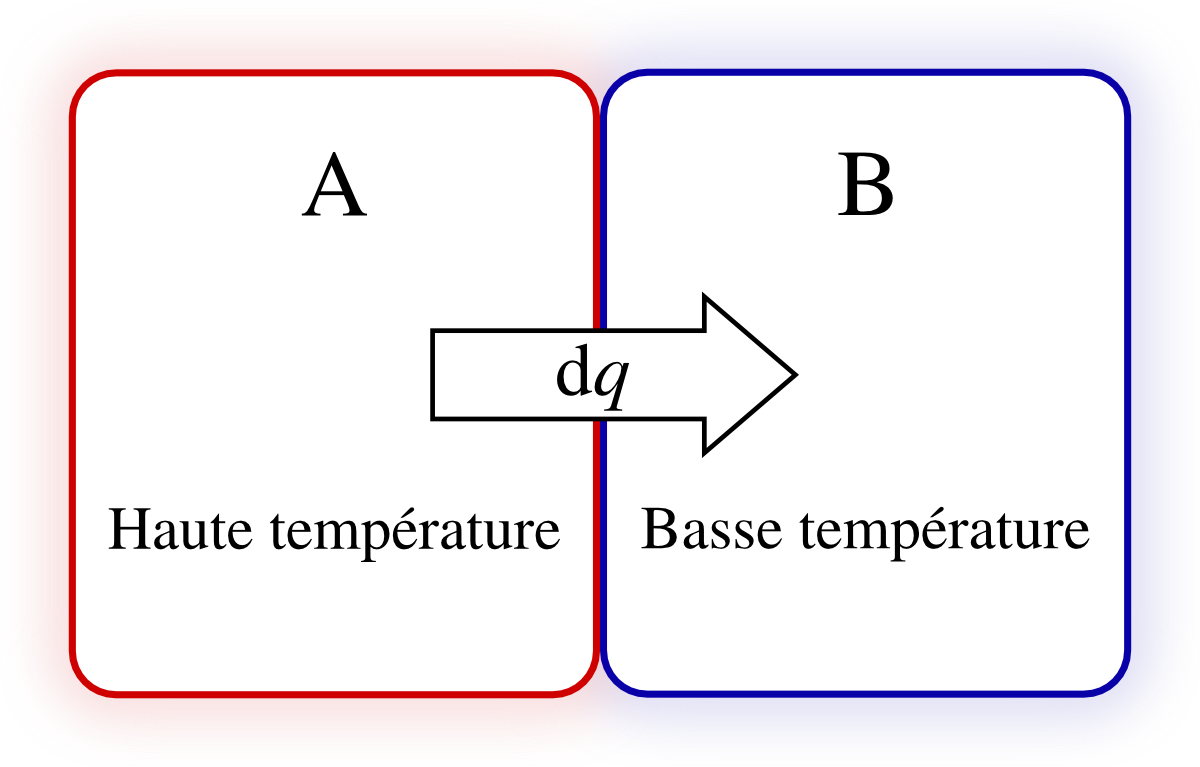
\includegraphics[width=8cm]{images/transfert_chaleur_irreversible.png}
			\end{center}
			\supercaption{Création d’entropie par transfert de chaleur. La transformation est réversible intérieurement pour chacun des deux corps A et B, mais irréversible pour le système [A+B].}{schéma \cczero \oc}
			\label{fig_expérience_création_entropie}
		\end{figure}


		Si nous supposons que la température du corps A est homogène\footnote{Cette «~supposition~» est parfaitement valide dans le cas où $\diff q$ est infiniment petit. Une intégration permettrait de prendre en compte la variation de température de A au cours de l’échange de chaleur, et le raisonnement ne serait pas modifié.},	sa perte de chaleur se fait de façon réversible. Ainsi la variation d’entropie de A est :
		\begin{equation*}
			\diff s_\A = - \frac{\diff q}{T_\A}
		\end{equation*}

		De même, on peut considérer que la température du corps B est homogène : son évolution est réversible intérieurement et la variation de son entropie est :
		\begin{equation*}
			\diff s_\B = + \frac{\diff q}{T_\B }
		\end{equation*}

		En revanche, la température du système entier [A+B] n’est pas du tout homogène : son évolution n’est pas réversible intérieurement. Même si l’ensemble ne reçoit aucune quantité de chaleur de l’extérieur, il n’a pas «~une~» température et nous ne savons pas lui appliquer l’intégrale~\ref{eq_variation_franche_entropie}, $\int_1^2 \left(T \diff s \right)_\text{rév.}$ pour calculer sa variation d’entropie. La variation de l’entropie du système [A+B] est la somme de celles de ses constituants, c’est-à-dire :
		\begin{equation}
			\diff s_{[A+B]} = \diff s_\A + \diff s_\B = \frac{\diff q}{T_\B } - \frac{\diff q}{T_\A}
		\end{equation}

		Comme $T_\A > T_\B$, cette variation est \emph{non-nulle} ; de l’entropie \emph{a été créée} lors du transfert thermique irréversible. L’irréversibilité n’a lieu ni dans la tasse A, ni dans la bouteille B, mais dans la fine frontière matérielle qui les sépare. L’évolution peut être représentée de manière plutôt convaincante sur un diagramme $T-s$ (\cref{fig_expérience_création_entropie_t-s}).

		\begin{figure}
			\begin{center}
				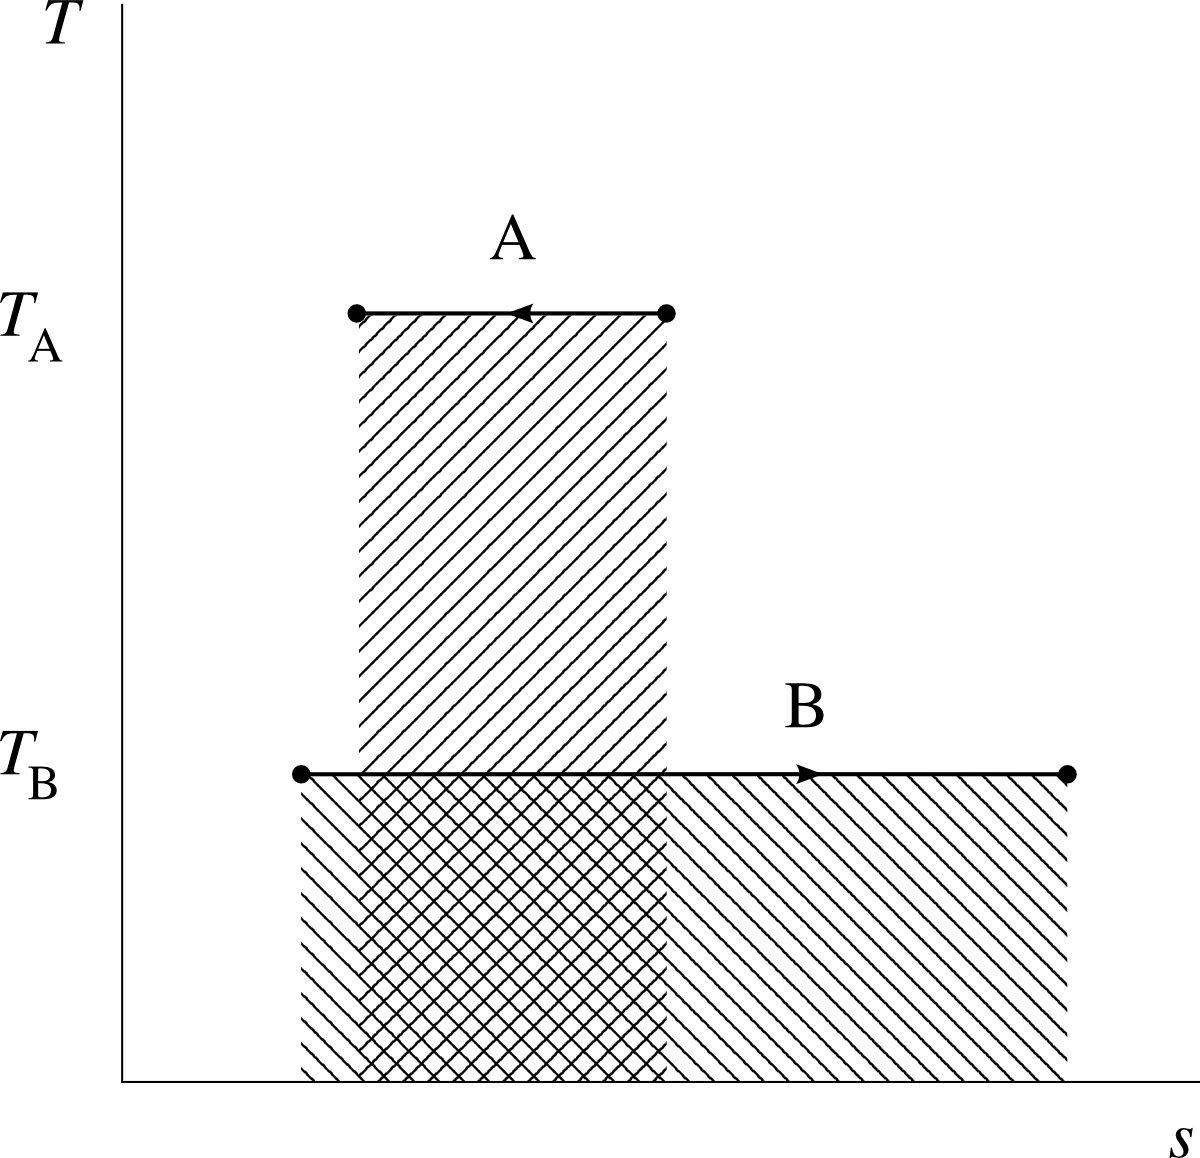
\includegraphics[width=\didacticpvdiagramwidth]{images/ts_echange_chaleur.png}
			\end{center}
			\supercaption{Variation d’entropie des corps A et B.
		Les deux aires hachurées sont égales (représentant la quantité de chaleur $\diff q$), mais la somme des deux entropies augmente.}{schéma \cczero \oc}
			\label{fig_expérience_création_entropie_t-s}
		\end{figure}

		\thermoquotebegin{0}
			\emph{Partout où il existe une différence de température, il peut y avoir production de puissance motrice}. Réciproquement partout où l’on peut consommer de cette puissance, il est possible de faire naître une différence de température, il est possible d’occasioner une rupture d’équilibre dans le calorique.
		\thermoquoteend{Sadi Carnot, 1824~\cite{carnot1824}}{}		
		Tout gradient de température donne lieu à une irréversibilité, et se traduit par une augmentation de l’entropie totale. \\
		On peut se représenter un flux de chaleur entre deux sources de températures différentes par une opportunité perdue de produire un travail -- ce qui sera sans doute source d’anxiété pour l’étudiant/e comme pour l’ingénieur/e. En plaçant une machine de Carnot entre les corps A et B, aucune irréversibilité n’aurait eu lieu et $\diff s_{[A+B]}$ serait nul. En plaçant une machine thermique de faible rendement, $\diff s_{[A+B]}$ serait faible ; le cas ci-dessus où le transfert de chaleur se fait sans machine est le cas limite où aucun travail n’est produit.\onlyframabook{\dontbreakpage}
		%http://soquij.qc.ca/fr/ressources-pour-tous/chroniques-linguistiques/ci-haut-et-ci-bas

	\subsection{Irréversibilités lors des compressions et détentes adiabatiques}

		Le deuxième type de transformation donnant lieu à des irréversibilités, et donc à une augmentation de l’entropie totale, est le transfert de travail dans les fluides.

		En pratique, toute détente ou compression se fait en présence d’irréversibilités internes. Comme la durée de l’évolution est finie (contrairement aux évolutions prescrites par Carnot), il y aura nécessairement des déséquilibres de pression au sein du fluide. Ces déséquilibres font apparaître de la turbulence interne, qui provoque la transformation d’énergie cinétique en chaleur, par frottement.

		Ainsi, une compression adiabatique réelle provoque plus d’échauffement du fluide qu’une compression adiabatique réversible (\cref{fig_t-s_détentes_compressions}) : une partie du travail fourni est entièrement convertie en chaleur, au travers des frottements internes.

		Par le même phénomène, une détente adiabatique réelle abaisse moins la température qu’une détente adiabatique réversible. À chaque fois, l’entropie est augmentée bien qu’aucun transfert de chaleur $\diff q$ n’ait eu lieu.
		
		\begin{figure}
			\begin{center}
				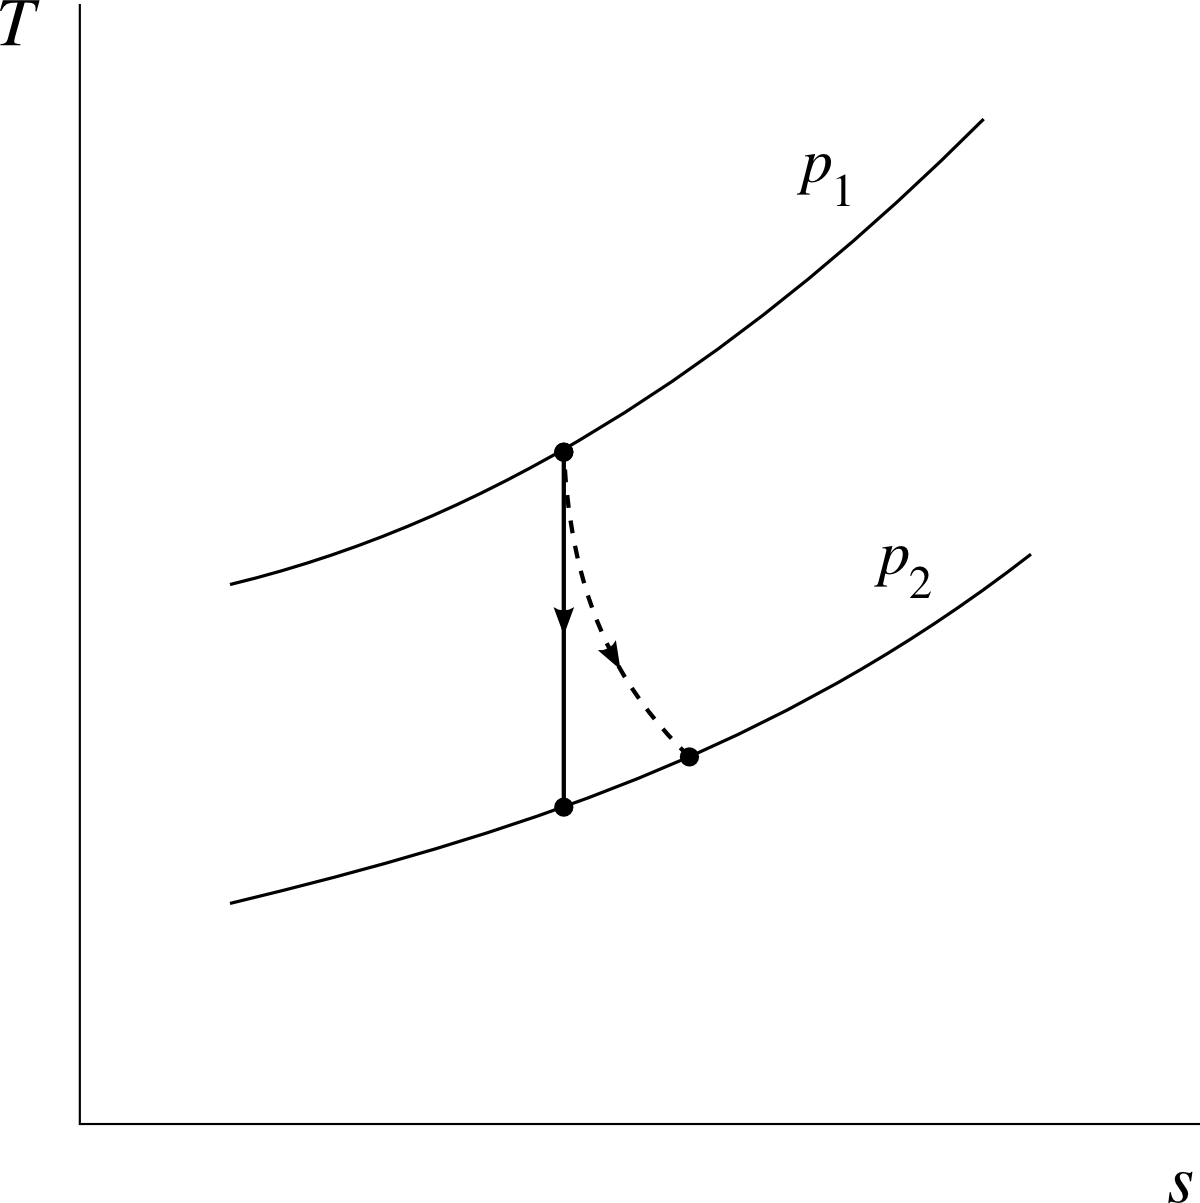
\includegraphics[width=0.48\textwidth]{images/ts_gp_detente.png}
				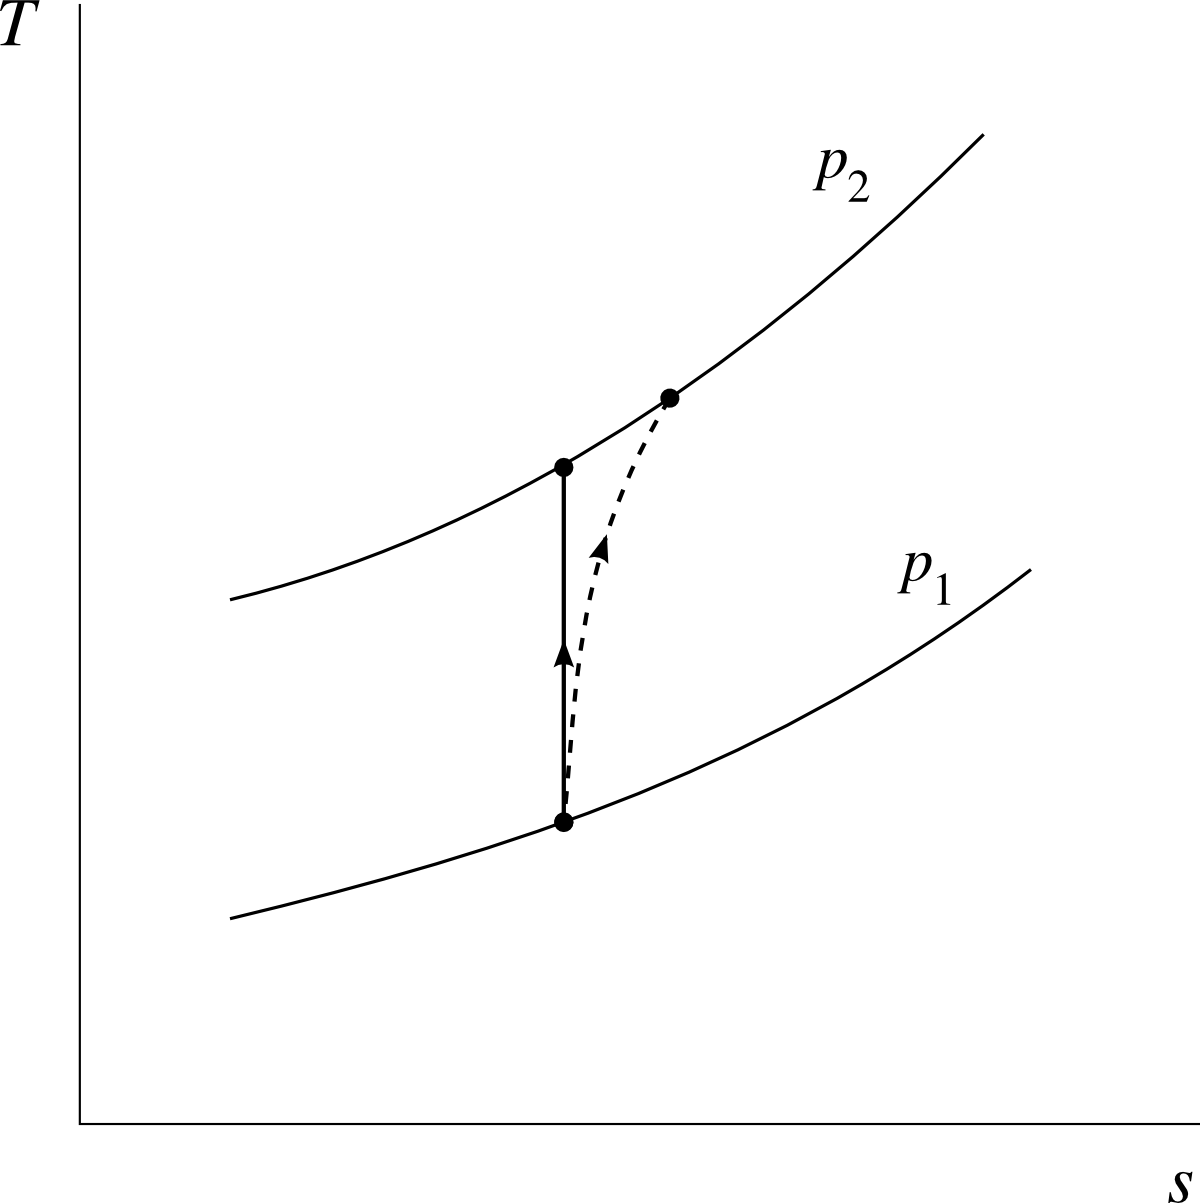
\includegraphics[width=0.48\textwidth]{images/ts_gp_compression.png}
			\end{center}
			\supercaption{Détente et compression adiabatiques théoriques (isentropiques, traits continus)
		et réelles (traits pointillés).\\
		Il faut bien noter que l’accroissement de l’entropie n’est en rien lié à un transfert de chaleur «~$\diff q$~». Le parcours sur le diagramme $T-s$ n’est pas continu et l’aire en dessous ne représente pas un flux de chaleur au travers des frontières du système.}{schéma \cczero \oc}
			\label{fig_t-s_détentes_compressions}
		\end{figure}

		

	\subsection{Le second principe et l’entropie}

		\thermoquotebegin{O}
			\emph{La chaleur ne peut passer d’un corps plus froid vers un corps plus chaud, sans qu’un changement en connection avec ce transfert n’ait lieu simultanément.}
			%en principe "connexion" en français, je ne sais pas si c'est "connection" dans la traduction que tu utilises.
		\thermoquoteend{Rudolf Clausius, 1854~\cite{clausius1854,clausius1867en,clausius1868fr4}}{}
		Nous avons admis au \courssept que la chaleur ne se déplaçait spontanément que vers une température plus basse --\ un postulat que nous nommons \textit{second principe}. Nous pouvons maintenant formuler cette affirmation avec une expression mathématique.
	
		\begin{description}
			\item[Lors d’un échange de chaleur] d’un corps à température $T_A$ vers un autre à température $T_B$, la variation globale d’entropie $\Delta s = \frac{-q}{T_\A} + \frac{q}{T_\B }$ est nécessairement nulle ou positive car $T_A$ est nécessairement égale ou supérieure à $T_B$.
			
			\item[Lors d’un échange de travail] toute irréversibilité donne lieu à une température finale plus haute qu’elle n’aurait pu l’être (cf. \S\ref{ch_évolutions_irr_sf}). L’obtention du même état final avec un chemin réversible demande donc un apport de chaleur, c’est-à-dire un terme $\int \left(\frac{\diff Q}{T}\right)_\text{rév.}$ positif. Une irréversibilité se traduit donc par une augmentation de l’entropie globale.
			
		\end{description}

		Ainsi, nous pouvons traduire le second principe de la façon suivante :
			
		\begin{trucimportant}
			Lorsqu’un système dont l’énergie est constante évolue,
				\begin{equation}
					\Delta s \geqslant 0
					\label{eq_augmentation_entropie}
				\end{equation}
		\end{trucimportant}

		On peut toujours réduire l’entropie d’un système pour la ramener à sa valeur initiale (il suffit pour cela de ramener le système lui-même à son état initial, quelle que soit la manière de procéder), mais cela se fera nécessairement au prix d’une augmentation \emph{au moins aussi grande} de celle d’un autre système.

	\subsection{Prédire le sens des transformations}
	
		Si l’on veut montrer qu’un système ne peut aller que d’un état A à un état B, c’est-à-dire que l’évolution est irréversible, il nous faut procéder de la façon suivante :
	
		\begin{enumerate}
			\item Il faut trouver un chemin réversible $\A \to \B$, c’est-à-dire un procédé pour aller de A à B en gardant toujours la pression et la température homogènes même si elles varient ;
			\item Le long de ce chemin réversible, nous calculons $\Delta s$ (c’est-à-dire que nous effectuons l’intégrale $\int \frac{\diff q}{T} $ pour ce chemin).
			\item Nous comparons avec l’intégrale $\int \frac{\diff q}{T} $ le long du chemin \emph{réel}, qui elle ne correspond pas à la variation d’entropie.
		\end{enumerate}

		Il y a trois possibilités :
			\begin{itemize}
				\item Si les deux intégrales sont égales, alors la transformation réelle est \vocab{réversible} : elle peut avoir lieu dans les deux sens.
				\item Si $\int \left(\frac{\diff q}{T}\right)_\text{chemin réel} < \int \left(\frac{\diff q}{T}\right)_\text{rév.}$, alors la transformation réelle est \vocab{irréversible}. Elle ne peut avoir lieu que dans ce sens.
				\item Si $\int \left(\frac{\diff q}{T}\right)_\text{chemin réel} > \int \left(\frac{\diff q}{T}\right)_\text{rév.}$, alors la transformation «~réelle~» décrite est \vocab{impossible}. Elle ne peut avoir lieu que dans le sens inverse (B $\to$ A). 
			\end{itemize}
		
		Nous pouvons donc, au moins pour quelques cas simples, retrouver mathématiquement le sens du temps -- une subtilité que l’on n’attendait pas de la part d’ingénieurs préoccupés par leur consommation de combustible !

		\begin{anexample}
			Une masse d’air suit une évolution sans apport de chaleur. Il y a deux états :
				\begin{itemize}
					\item Un état $X$ à~\SI{5}{\bar} et~\SI{100}{\degreeCelsius} ;
					\item Un état $Y$ à~\SI{1}{\bar} et~\SI{5}{\degreeCelsius}.
				\end{itemize}
			Quel est le seul sens ($X \to Y$ ou $Y \to X$) dans lequel l’évolution peut avoir lieu ?
						
				\begin{answer}
					Proposons le sens $X \to Y$ et vérifions s’il est physiquement possible.
					
					La variation d’entropie est égale à l’intégrale $\int_X^Y \left(\frac{\diff q}{T}\right)_\text{rév.}$. Avec l’\cref{eq_delta_s_gp_p}, $\Delta s = c_p \ln \frac{T_Y}{T_X} - R \ln \frac{p_Y}{p_X} = \num{1005} \ln \frac{5+273,15}{100+273,15} - \num{286} \ln\frac{1}{5}=  \SI{+166,6}{\joule\per\kelvin\per\kilogram}$.

					De l’autre côté, l’intégrale $\int_X^Y \left(\frac{\diff q}{T}\right)_\text{chemin réel}$ est égale à zéro car en réalité il n’y a pas eu de transfert de chaleur ($\diff q = 0$).
					
					Nous avons donc $\Delta s > \int_X^Y \left(\frac{\diff q}{T}\right)_\text{chemin réel}$ et l’évolution est irréversible. Si nous voulions revenir en arrière, de $Y$ à $X$, nous serions obligés de retirer de la chaleur.
					
					L’évolution peut être représentée de façon qualitative sur un diagramme $T-s$ ainsi :
						\begin{center}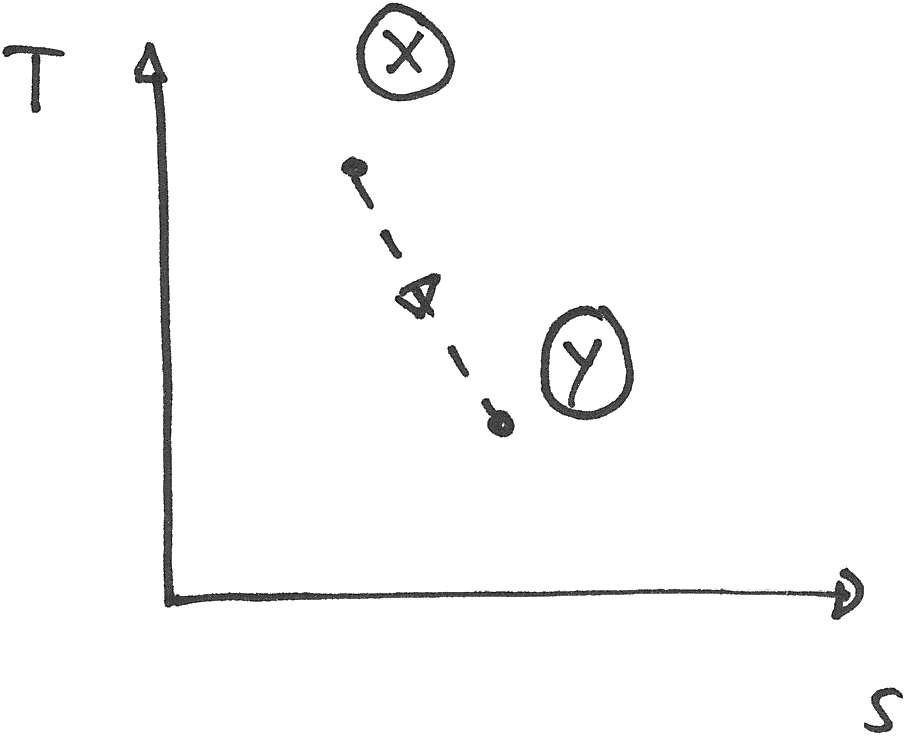
\includegraphics[width=4cm]{images/exe_ts_7.png}\end{center}
				\end{answer}
		\end{anexample}

		

		\begin{anexample}
			De l’eau suit une évolution pendant laquelle on lui apporte \SI{1}{\mega\joule\per\kilogram} de chaleur (sa température étant alors figée à~\SI{130}{\degreeCelsius}). Il y a deux états, un au début et l’autre à la fin :
				\begin{itemize}
					\item Un état $X$ à l’état de liquide saturé à~\SI{130}{\degreeCelsius} ;
					\item Un état $Y$ à l’état de vapeur saturée à~\SI{170}{\degreeCelsius}.
				\end{itemize}
			Quel est le seul sens ($X \to Y$ ou $Y \to X$) dans lequel l’évolution peut avoir lieu ?
						
				\begin{answer}
					Proposons le sens $X \to Y$ et vérifions s’il est physiquement possible.
					
					Nous lisons les valeurs de l’entropie dans l’abaque n°2 : $s_X = s_{L \SI{130}{\degreeCelsius}} = \SI{1,6346}{\kilo\joule\per\kelvin\per\kilogram}$ et $s_Y = s_{V \SI{170}{\degreeCelsius}} = \SI{6,665}{\kilo\joule\per\kelvin\per\kilogram}$. \\
					Ainsi, $\Delta s = \int_X^Y \left(\frac{\diff q}{T}\right)_\text{rév.} = \SI{+5,03}{\kilo\joule\per\kelvin\per\kilogram}$.
					
					De l’autre côté, nous pouvons calculer l’intégrale $\int_X^Y \left(\frac{\diff q}{T}\right)_\text{chemin réel}$ car nous savons que la chaleur a été apportée lorsque la température était fixée à~\SI{130}{\degreeCelsius}. Ainsi $\int_X^Y \left(\frac{\diff q}{T}\right)_\text{chemin réel} = \frac{1}{T} \int_X^Y \left(\diff q\right)_\text{chemin réel} = \frac{q_{X\to Y}}{T} = \frac{\num{1e6}}{170+273,15} = \SI{+2,26}{\kilo\joule\per\kelvin\per\kilogram}$.
					
					L’évolution peut être représentée de façon qualitative sur un diagramme $T-s$ ainsi :
						\begin{center}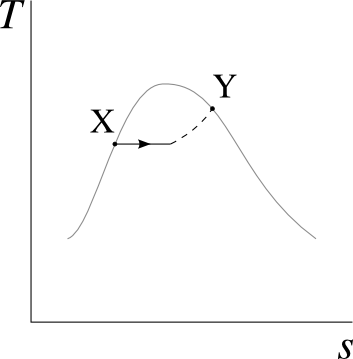
\includegraphics[width=4cm]{images/exe_ts_8.png}\end{center}
					
					Ici, nous avons $\Delta s > \int_X^Y \left(\frac{\diff q}{T}\right)_\text{chemin réel}$ et l’évolution est irréversible. Si nous voulions revenir en arrière, de $Y$ à $X$, nous serions obligés de refroidir le gaz en lui retirant \emph{nécessairement} une quantité plus grande que \SI{1}{\mega\joule\per\kilogram}.
				
				\end{answer}
		\end{anexample}

\section{L’entropie, le temps, et l’univers}

	\subsection{L’entropie pour l’ingénieur}

		Nous avons vu que l’entropie, de la même façon que l’énergie, est un concept dont la quantification des variations permet de déterminer les transformations qui sont \emph{possibles}. Il s’agit donc fondamentalement d’un concept de physicien/ne. Pour l’ingénieur/e, l’entropie est :
		\begin{itemize}
			\item «~ce qui ne varie pas lorsque l’on comprime et détend les fluides de façon idéale~». Ainsi la quantification de $\Delta s$ nous permet de quantifier les propriétés que devrait avoir un fluide à la sortie d’un compresseur ou d’une turbine ;
			\item «~ce qui ne varie pas lorsque l’on transfère de la chaleur à l’intérieur d’un système de façon idéale~». Ainsi la quantification de $\Delta s$ nous permet de calculer l’irréversibilité qui a lieu lors des échanges de chaleur.
		\end{itemize}

	À chaque fois que nous donnons lieu à une augmentation de l’entropie globale, il nous faut au final effectuer un rejet de chaleur indésirable. Ainsi, ces quantifications de $\Delta s$ nous permettent de mesurer la qualité des détentes, compressions, refroidissements et réchauffements que nous effectuons avec les fluides dans nos machines.

	\subsection{Contexte : le sens du temps}
				
		Les exemples que nous avons étudiés dans ce chapitre pour déterminer le sens des transformations sont très académiques, toutefois la démarche reste valide pour toute transformation : une pierre jetée dans un étang, une assiette qui se casse en tombant, etc. Si nous revenons aux trois photos de la~\cref{fig_water_jump}, nous pourrions en retrouver l’ordre en déterminant les états initial et final de l’eau autour de la plongeuse, et en comparant $\Delta s$ à l’intégrale $\int \left(\frac{\diff q}{T}\right)_\text{chemin réel}$ réalisée pendant l’entrée dans l’eau. 
		
		C’est ce désir de retrouver l’ordre absolu dans lequel se succèdent les états, c’est-à-dire le sens du temps, qui a mené le physicien allemand \wf{Rudolf Clausius} jusqu’à proposer le concept d’\vocab{entropie} en 1865 dans une publication magistrale --\ \textit{Über verschiedene für die Anwendung bequeme Formen der Hauptgleichungen der mechanischen Wärmetheorie}~\cite{clausius1865,clausius1867en,clausius1868fr2}. Concluant une décennie de travail autour de la grandeur $\frac{Q}{T}$, il y formalise un concept que ses condisciples français \wf{Ferdinand Reech} et écossais \wf{William Rankine} n’avaient qu’effleuré~\cite{truesdell1980}, et y rassemble l’ensemble des connaissances contemporaines de sa discipline.
		
		\thermoquotebegin{O}
			\onlyamphibook{\vspace{-0.5cm}\par}%handmade
			J’ai intentionnellement formé le mot \vocab{entropie} de sorte qu’il soit aussi similaire au mot \vocab{énergie} que possible, parce que les sens physiques des deux grandeurs nommées par ces mots sont si étroitement liées qu’il m’a semblé qu’une cetraine similarité dans leurs désignations était désirable.
		\thermoquoteend{Rudolf Clausius, 1865~\cite{clausius1865,clausius1867en,clausius1868fr2}}{}
		Clausius forge le mot \textit{en-tropie} à partir du grec ancien \textgreek{ἡ-τροπή}, \textit{changement interne}, ce qui, couplé à son ton autoritaire, ne fait rien pour gagner l’enthousiasme de ses contemporains. Mais le concept est si puissant, et l’\cref{eq_augmentation_entropie} si simple, qu’ils sont universellement acceptés.
		
		Ainsi, après un siècle d’efforts, la physique de la chaleur a rattrapé la technologie des moteurs. Nous voilà capables de décrire entièrement et de façon quantitative le comportement des corps sans devoir nous pencher sur celui de leurs constituants, tels que les molécules, atomes ou particules sub-atomiques : l’entropie était la dernière pièce manquante de ce que nous appelons aujourd’hui la \vocab{thermodynamique macroscopique}.
		
		
	\subsection{L’entropie à l’échelle microscopique}
	\label{ch_entropie_boltzmann}
	
		Passé Clausius, le développement de la thermodynamique n’intéresse plus guère les ingénieurs, mais les physiciens ne sont pas rassasiés. Il nous reste en effet un problème, car si nous avons bien \emph{décrit} le phénomène d’irréversibilité, nous n’avons toujours pas \emph{expliqué} son origine à l’intérieur de corps constitués de particules dont les évolutions (un incessant bourdonnement de collisions, à base de forces d’attraction et de répulsion), \emph{elles}, sont parfaitement réversibles.
		
		Il ne faudra que dix ans pour que la réponse soit formalisée : l’autrichien \wf{Ludwig Boltzmann} propose en 1875 une \vocab{définition microscopique} de l’entropie :
			\begin{equation}
				S \equiv k \ln \lambda
			\end{equation}
			\begin{equationterms}
				\item où \tab $\lambda$ \tab est le nombre de configurations possibles du système qui correspondent à son état, 
				\item et \tab $k$ \tab est une constante.
			\end{equationterms}
		
		\thermoquotebegin{O}
		Nous mesurons le «~dés\-or\-dre~» par le nombre de manières dont l’intérieur peut être arrangé, de telle sorte que de l’extérieur cela apparaisse la même chose. \emph{Le logarithme de ce  nombre de manières est l’entropie}.\\
Ainsi, avec la définition technique ci-dessus du désordre, nous pouvons comprendre la proposition. Premièrement, l’entropie mesure le désordre. Deuxièmement, l’univers va toujours de «~l’ordre~» vers le «~désordre~», ainsi l’entropie augmente toujours. L’ordre n’est pas un ordre au sens où nous aimons l’arrangement, mais au sens où le nombre de manières différentes à notre disposition pour obtenir quelque chose de toujours extérieurement identique, est relativement restreint. 
		\thermoquoteend{Richard Feynman, 1963~\cite{feynman1963, feynman1963fr}}{}
		Ainsi pour Boltzmann l’entropie est une mesure de la probabilité du système d’être dans cet état. Plus la configuration est probable (homogénéité de la pression et de la température), plus l’entropie est grande. 
		
		À l’échelle macroscopique, nous avions décrit le second principe comme une impossibilité (\S\ref{ch_second_principe_enonce}) : un objet de température homogène ne peut pas voir spontanément une extrémité se refroidir et l’autre se réchauffer. Selon Boltzmann, un tel événement n’est pas strictement impossible, mais seulement très improbable. L’état où les molécules les plus rapides sont toutes rassemblées à une extrémité, et les plus lentes à l’autre, est bien moins probable (entropie plus faible) qu’un état où elles sont réparties de façon homogène (entropie plus grande).
		
		Cette approche a non seulement le mérite de raccrocher notre discipline avec la théorie atomique --\ et nous parlerons dès lors de \vocab{thermodynamique microscopique} et \vocab{statistique}\ -- mais elle va aussi ouvrir la porte de la théorie de l’information. En effet, la résolution et la précision avec lesquelles on évalue l’état d’un système affectent le nombre de configurations possibles que l’on peut lui attribuer. Voici le concept de l’\vocab{information} rattaché à d’autres propriétés physiques : un résultat impressionnant pour une discipline qui ne visait qu’à explorer ce que voulait dire~«~chaud~» !
		
	\subsection{L’entropie et l’univers}
	
		\thermoquotebegin{O}
			Pendant une durée de temps finie dans le passé, la terre a du être --et dans une durée de temps à venir elle devra l’être encore-- impropre à l’habitat de l’homme tel qu’il est présemment constitué, à moins que des opérations aient été ou soient réalisées qui sont impossibles selon les lois qui régissent les opérations ayant lieu aujourd’hui dans le monde matériel.
		\thermoquoteend{William Thomson, 1852~\cite{kelvin1852}}{}
		Nous quittons l’entropie sur une question ouverte. Dans la mesure où l’on pense l’univers comme étant un ensemble fini, c’est-à-dire comme à un système isolé contenant une quantité fixe d’énergie, peut-on lui appliquer l’\cref{eq_augmentation_entropie} : $\Delta s_\text{univers} > 0$ lorsque le temps passe ? L’univers tend-il vers une température minimale homogène finale ? Clausius est sans équivoque : il termine aussitôt son article de 1865 par l’affirmation :
			
			\begin{quote}
				Si l’on imagine que l’on ait calculé d’une manière conséquente pour l’univers entier […] la quantité que j’ai nommée \vocab{entropie} pour un corps particulier, ainsi que la quantité désignée sous le nom d’\vocab{énergie} et dont le sens est plus facile à saisir, on pourra exprimer très simplement, sous la forme suivante, les lois fondamentales de l’univers qui correspondent aux deux principes essentiels de la théorie mécanique de la chaleur :
					\begin{enumerate}
						\item L’énergie de l’univers est constante.
						\item L’entropie de l’univers tend vers un maximum.
					\end{enumerate}
			\end{quote}
		
		La théorie des réfrigérateurs et des moteurs est-elle apte à prévoir la fin du monde ? Pour explorer cette question de façon ludique, l’étudiant/e pourra lire \textit{L’ultime question} d’Isaac \mbox{Asimov}~\cite{asimov1956,asimov1956fr} ou \textit{L’entropie et tout ça} de Philippe \mbox{Depondt}~\cite{depondt2001}. Pour une réponse plus formelle, il faudra se reporter à un bon manuel de physique.
